%	Sottolineare il target di tecnologie per cui è effettuata la progettazione. Queste non verranno citate all'interno del capitolo
%	di Progetto ma, il seguente capitolo di Realizzazione, introducendo banalmente le tecnologie utilizzate, dovrà poter
%	calzare perfettamente e dovrà facilmente potersi riallacciare a quanto detto in questo capitolo.

%	In questa sezione si ripercorrono gli stessi argomenti della parte di analisi, in parallelo, ma focalizzandosi sulle scelte di
%	progetto. Queste dovranno essere motivate e lo scopo di questa porzione di testo è di definire le varie parti e la loro 
%	collaborazione GLOBALE (API + persistenza). Il livello di dettaglio non sarà massimo in quanto nelle successive sezioni 
%	si entrerà nello specifico.
%
%	{Diagrammi} Class diagrams UML o analoghi più efficaci per il comportamento dinamico

	A seguito della fase di analisi appena condotta, si passa all'ambito più strettamente progettuale. Scopo di questa sezione introduttiva è quello di riallacciarsi ai requisiti già esposti in fase di analisi, aggiungendo obiettivi di progettazione. Per quanto riguarda le API, si è già parlato dei requisiti funzionali, cosi come si è sottolineata la necessità di utilizzo in \textit{concorrenza}. Una trattazione più dettagliata è operata in fase di analisi. Si pone l'accento invece su alcuni obiettivi progettuali di cui si è tenuto conto:
	
	\begin{enumerate}
		\item \textbf{Prestazioni}. Si vogliono garantire complessità computazionali compatibili e coerenti con quelle illustrate in fase di analisi per la Skip List, minimizzando lo spazio usato dalla struttura dati, cosi come garantire ottimi tempi di risposta e throughput.
	  	\item \textbf{Usabilità}. Si vuole una interfaccia ben definita, chiara, di facile interpretazione e stabile, al fine di ottimizzarne l'utilizzo.
	  	\item \textbf{Sostenibilità}. Progettazione e realizzazione devono permettere alti livelli di manutenibilità per poter operare ottimizzazioni, miglioramenti e riparazioni. Di pari importanza sono la verificabilità e la configurabilità delle API.
	\end{enumerate}
	 
	Per quanto riguarda la sezione sulla persistenza, invece, si ricordano i due requisiti fondamentali. Il primo riguarda la trattazione della stessa come un'estensione delle API, il secondo invece sottolinea la caratteristica di trasparenza dell'introduzione di questa estensione, rispetto alla libreria stessa.
	Si pone anche qui l'accento sugli obiettivi progettuali principali di cui si è tenuto conto:
	
	\begin{enumerate}
		\item \textbf{Efficienza}. L'obiettivo principale riguarda l'impostazione della restituzione e caricamento di elementi da e sul database in maniera parallela piuttosto che sequenziale. Inoltre è auspicabile un sistema che sappia lavorare sul minimo di informazioni necessarie all'esecuzione delle operazioni, evitando il più possibile traffico di elementi inutili. L'architettura complessiva, infine, dovrebbe poter lavorare con un sistema di caching efficiente, per ridurre il traffico di informazioni generale e dunque il carico gravante sulle query con il database.
		\item \textbf{Affidabilità}. Si vuole un sistema disponibile, sempre attivo e che fornisca la capacità di essere ripristinato a seguito di guasti, errori o fallimenti.
	\end{enumerate}

	Seguono i diagrammi della classi dell'intera progettazione per fornire un contesto alla successiva analisi dettagliata delle singole parti\footnote{Per tutti i diagrammi delle classi mostrati, la molteplicità delle varie associazioni è sottintesa essere pari a 1.}.

	\begin{figure}
		\centering
		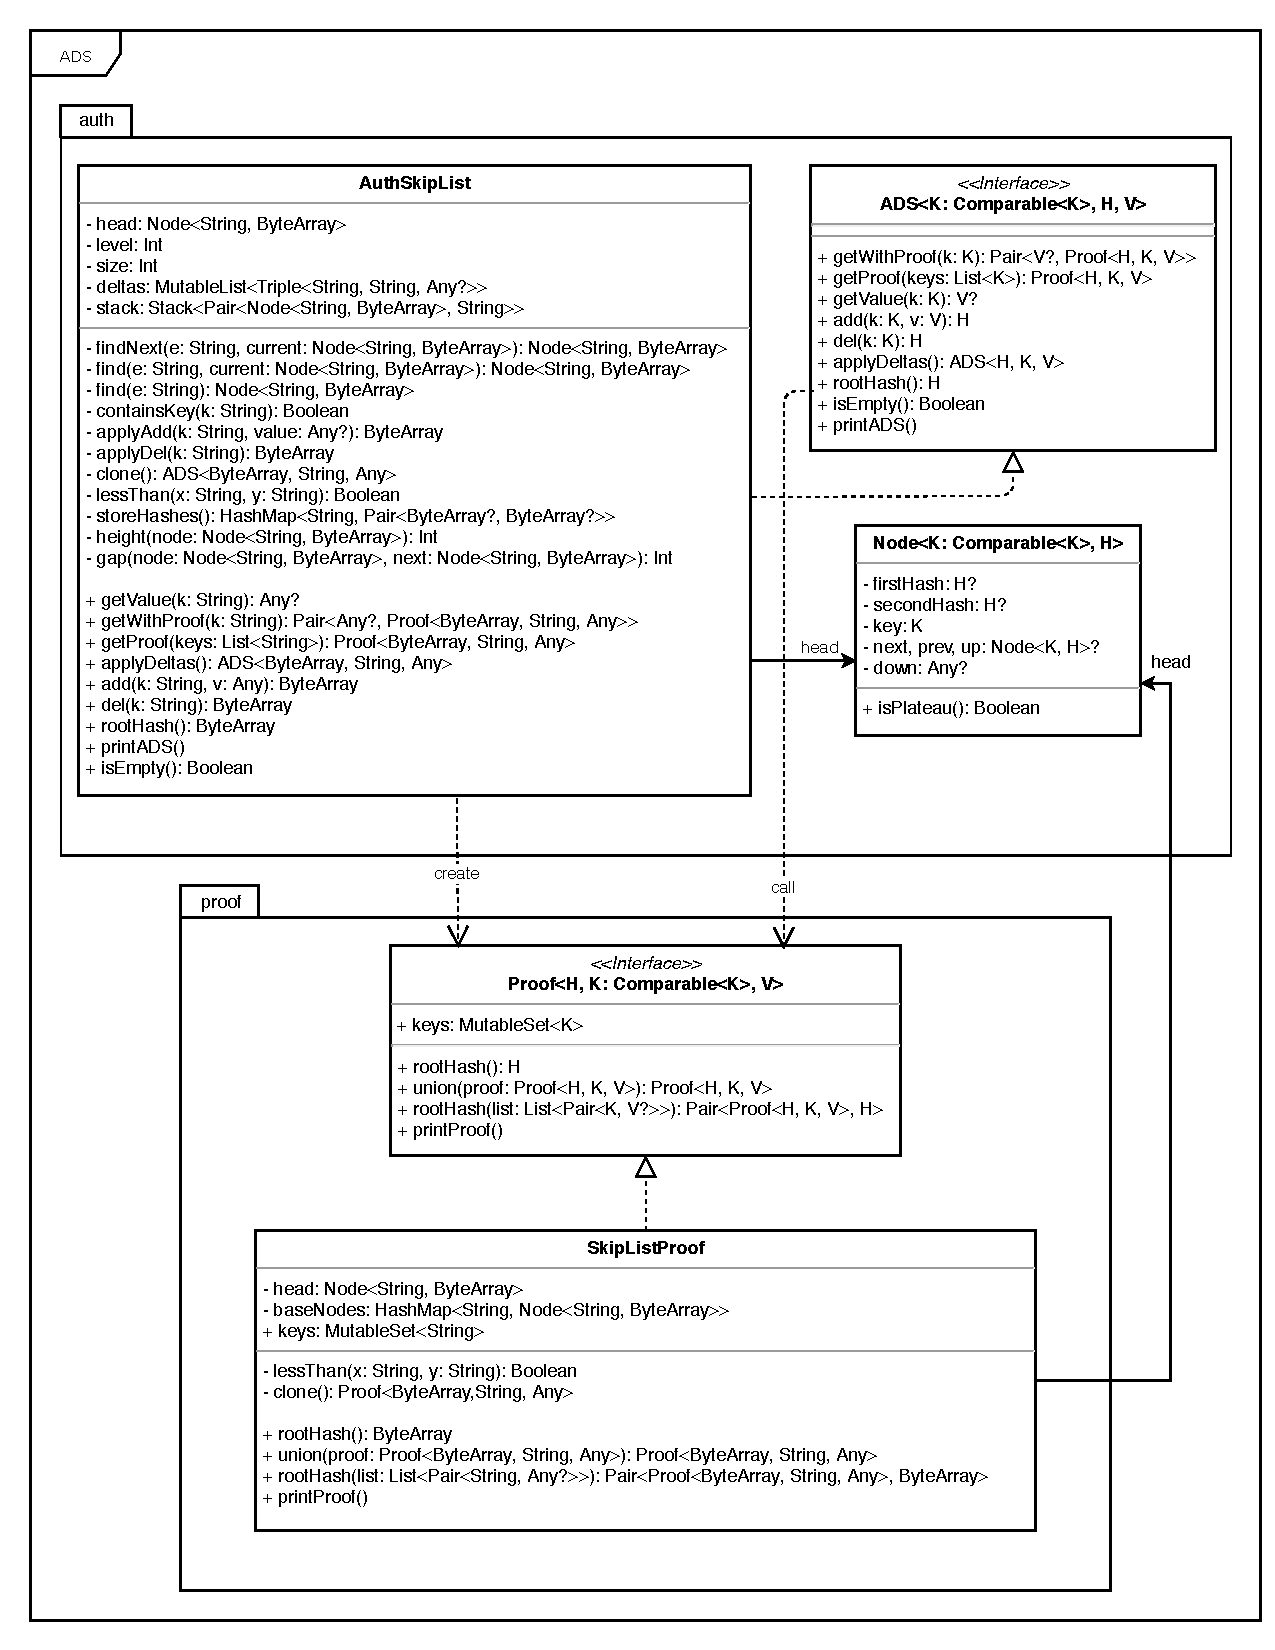
\includegraphics[scale=0.65]{figure/Auth+Proof.pdf}
		\caption{Diagramma delle classi di progetto per la parte di autenticazione. Con un piccolo abuso di notazione sono stati presi in prestito alcuni elementi sintattici dal linguaggio \textit{Kotlin}, con cui sono state realizzate le API.}\label{fig:authDCD}
	\end{figure}

	\begin{figure}
		\centering
		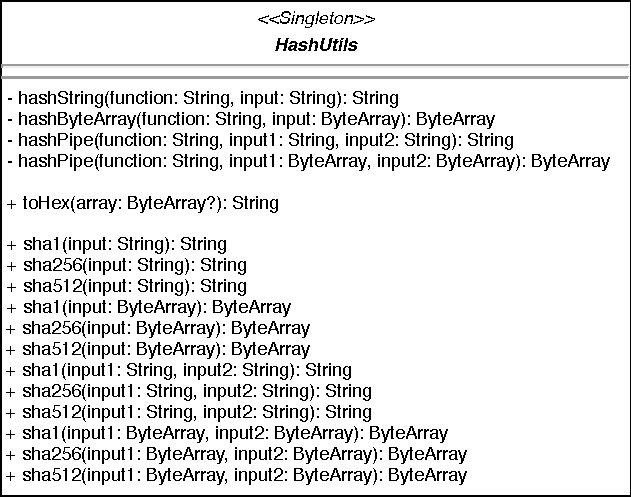
\includegraphics[scale=0.65]{figure/HashUtils.pdf}
		\caption{\textit{Singleton} per funzioni di utilità per calcolo e restituzione di hash.}\label{fig:hashUtils}
	\end{figure}

	\begin{figure}
		\centering
		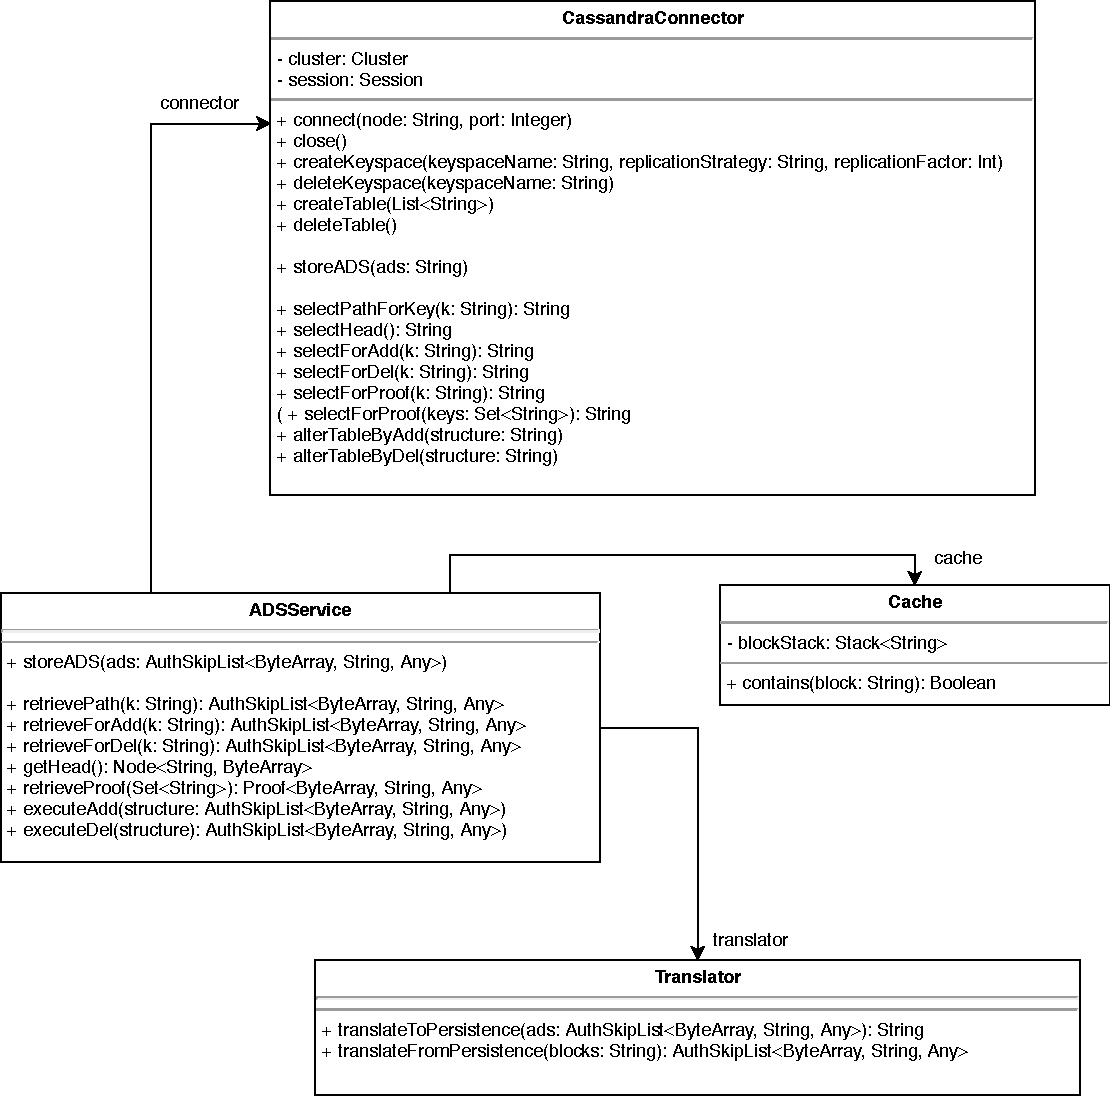
\includegraphics[scale=0.65]{figure/ServiceDCD.pdf}
		\caption{Diagramma delle classi di progetto per la parte di persistenza.}\label{fig:ServiceDCD}
	\end{figure}

\section{API}

%	{Analisi prettamente tecnologica}
%	
%	Qui, sulla base di quanto detto nella sezione di analisi, si inizia a mettere insieme le varie parti per descrivere più
%	nel dettaglio l'API dal punto di vista progettuale. Già nella prima parte di analisi è stato introdotto a grandi linee il funzionamento.
%	
%	Il focus è sulle scelte progettuali. Evidenziare dunque le scelte a livello di pattern.

	Come già deducibile dal Class Diagram in figura~\ref{fig:authDCD}, le API consistono fondamentalmente di due interfacce, \textit{stabili}, \textit{comuni} e \textit{unificate}, che forniscono \textit{Protected Variation} rispetto a rivisitazioni e ottimizzazioni. Pertanto è stato fornito all'utilizzatore un punto di contatto singolo, una \textit{Facade}, con le librerie. 
	Le implementazioni di queste due interfaccie sono soggette a due vincoli di progetto riguardanti il tipo da utilizzare per le chiavi, ovvero una stringa di caratteri, e per gli hash, ovvero array di byte e/o stringa di caratteri. Esse di basano entrambe sul \textit{Node} come elemento costituente di base. Per le funzioni di hash, esse si affidano ad un \textit{Singleton} di utilità, HashUtils. Prima di passare ad un'analisi dettagliata delle varie parti, si sottolinea la dipendenza della Skip List Autenticata all'interfaccia della Proof, e \textit{non} alla sua implementazione. Questo è stato preferito, fornendo uno strato di \textit{Indirection}, in quanto la Skip List Proof, può subire cambiamenti e ottimizzazioni interne, senza ripercuotersi direttamente sulla Skip List Autenticata.
	Nei successivi paragrafi si spiegherà più nel dettaglio ogni parte attiva all'interno del progetto di queste API, illustrandone e motivandone tutte le scelte progettuali rilevanti.
	
	\subsection{Interfaccia ADS}
	
	%	MODELLO FUNZIONALE, motivare la necessità
	%
	%	Sezione in cui si motiva pattern per interfaccia e si evidenzia collegamento funzionale con casi d'uso e requisiti, in termini solo di funzionalità offerte
	
		L'interfaccia dell'ADS, è stata resa parametrica rispetto a tre valori:
		
		\begin{itemize}
			\item \textbf{H}: il tipo dei vari \textit{hash} presenti all'interno dei nodi della struttura.
			\item \textbf{K}: il tipo delle \textit{chiavi} dei nodi.
			\item \textbf{V}: il tipo dei valori presenti nello \textit{storage}. 
		\end{itemize}
	
		Questa scelta rende l'interfaccia applicabile parametricamente rispetto alla scelta dei suddetti tipi, caratteristica utile per garantire flessibilità. 

		Le operazioni fornite dall'ADS, sulla base di requisiti e casi d'uso già discussi in fase di analisi, sono:
		\begin{itemize}
			\item \textbf{\textit{getWithProof(k: K): Pair<V?\footnote{Il punto interrogativo accanto ad un parametro sta ad indicare che quel parametro può essere anche nullo}, Proof<H, K, V>>}}: restituisce il valore $ v $ associato alla chiave $ k $, assieme alla \textit{Proof} per quella chiave. Questa operazione è necessaria per permettere di ottenere la Proof relativa ad una specifica coppia chiave-valore $ (k,v) $.
			\item\textbf{ \textit{getProof(keys: List<K>): Proof<H, K, V>}}: restituisce la Proof relativa alle chiavi contenute nella lista \textit{keys}. Estende le possibilità di \textit{getWithProof(k)}, restituendo in un solo round una Proof cumulativa per un'insieme di chiavi $ keys $, valida e utilizzabile per tutte le stesse. 
			\item \textbf{\textit{getValue(k: K): V?}}: data una chiave $ k $, restituisce il valore $ v $ associato ad essa. Questa operazione permette dunque le operazioni di lettura, \textit{read(k)}, richieste dai casi d'uso.
			\item \textbf{\textit{add(k: K, v: V): H}}: crea un \textit{delta} rispetto alla struttura corrente, il quale viene memorizzato. Il delta riguarda l'aggiunta o la modifica degli elementi relativi alla chiave $ k $. L'operazione \underline{non} modifica la struttura corrente.
			\item \textbf{\textit{del(k: K): H}}: crea un \textit{delta} rispetto alla struttura corrente, il quale viene memorizzato. Il delta riguarda la cancellazione degli elementi relativi alla chiave $ k $ L'operazione \underline{non} modifica la struttura corrente.
			\item \textbf{\textit{applyDeltas(): ADS<H, K, V>}}: compatta tutti i vari delta relativi alla struttura corrente e li applica in ordine, restituendo una nuova ADS, con le modifiche applicate. Questa operazione permette all'ADS di avere la capacità di aggiornarsi rispetto a richieste di update in arrivo dai client.
			\item \textbf{\textit{rootHash(): H}}: calcola e restituisce il \textit{Root Hash} della struttura corrente. Questa operazione permette di ottenere il \textit{digest} dell'intera struttura, come specificato dai requisiti.
			\item \textbf{\textit{isEmpty(): Boolean}}: Informa se l'ADS è vuoto o meno.
		\end{itemize}
	
		E' necessario sottolineare riguardo alla prima operazione fornita, che, per \textit{Creator}, sara l'ADS stesso a generare una Proof una o più chiavi, proprio in quanto è l'unica entità a conoscere le informazioni per farlo. A seguito della creazione, essa sarà un entità indipendente, in grado di aggiornarsi in parallelo rispetto agli update. I calcoli e le operazioni poi eseguite sulla Proof, sono indipendenti dall'ADS di partenza.
		
		Di fondamentale importanza è il requisito relativo alla possibilità di utilizzo dell'ADS in ambito concorrente. Deve essere possibile, dunque, poter operare operazioni in parallelo sull'ADS, senza che ci siano conflitti dovuti alla concorrenza. Pertanto è stato deciso di applicare un principio tipico del paradigma di programmazione funzionale, secondo cui i valori non vengono trovati cambiando lo stato dell'ADS, ma costruendo nuovi stati a partire dai precedenti. Per questo motivo le operazioni di scrittura, ovvero quelle che modificherebbero lo stato della struttura, lo fanno in maniera totalmente compatibile con quanto detto. Una spiegazione più dettagliata di come questo sia stato realizzato è posticipata in paragrafi successivi.
		
		La scelta invece di disaccoppiare il momento dell'individuazione della operazioni di aggiunta, modifica o cancellazione, dal momento della loro effettiva applicazione, è da inquadrare in un contesto più ampio di utilizzo della libreria. Intuitivamente, questa funzionalità è fornita per permettere di gestire meglio gli stati in cui si può trovare la struttura stessa: ad esempio uno stato in cui può ricevere e accumulare update, piuttosto che uno stato in cui questi vengono applicati in blocco. Migliore è di conseguenza la gestione delle operazioni di lettura, in quanto per garantirne la consistenza, esse possono essere collocate in istanti temporali diversi, prima o dopo determinati stati della struttura.
		
		L'interfaccia, e dunque la classi che implementeranno quest'ultima, deve implementare a sua volta l'interfaccia \textit{Serializable}, in quanto dovrà avere la caratteristica di essere, appunto, serializzabile. Questo è motivato dal fatto che implementazioni di questa interfaccia saranno inserite all'interno di messaggi che dovranno essere spediti su rete, nell'ambito dell'utilizzo di questa API.
	
	\subsection{Interfaccia Proof}
	
	%	MODELLO FUNZIONALE, motivare la necessità
	%
	%	Sezione in cui si motiva pattern per interfaccia e si evidenzia collegamento funzionale con casi d'uso e requisiti, in termini solo di funzionalità offerte
		
		L'interfaccia della Proof, è stata resa parametrica rispetto a tre valori:
		
		\begin{itemize}
			\item \textbf{H}: il tipo dei vari \textit{hash} presenti all'interno dei nodi della Proof.
			\item \textbf{K}: il tipo delle \textit{chiavi} dei nodi.
			\item \textbf{V}: il tipo dei valori presenti nello \textit{storage}. 
		\end{itemize}
		
		Questa scelta rende l'interfaccia applicabile parametricamente rispetto alla scelta dei suddetti tipi, caratteristica utile per garantire flessibilità. 
		
		Le operazioni fornite dalla Proof, sulla base di requisiti e casi d'uso già discussi in fase di analisi, sono:
		\begin{itemize}
			\item \textbf{\textit{keys: Set<K>}}: insieme contenente tutte le chiavi per cui è valida la Proof.
			\item \textbf{\textit{rootHash(): H}}: restituisce il \textit{Root Hash} della Proof. Questa, assieme alla successiva, sono requisiti funzionali già discussi in fase di analisi.
			\item \textbf{\textit{rootHash(list: List<Pair<K, V>>): Proof<H, K, V>}}: applica gli aggiornamenti specificati nella lista di coppie chiave-valore \textit{list} e successivamente calcola e restituisce il nuovo \textit{Root Hash}.
			\item \textbf{\textit{union(proof: Proof<H, K, V>): Proof<H, K, V>}}: effettua il \textit{merge} di due Proof relative allo stesso istante temporale della stessa struttura da cui sono state generate. Restituisce una nuova proof, cumulativa rispetto a quelle di partenza.
		\end{itemize}
		
		Di fondamentale importanza è il requisito relativo alla possibilità di utilizzo della Proof in ambito concorrente. Deve essere possibile, dunque, poter operare operazioni in parallelo sulla Proof, senza che ci siano conflitti dovuti alla concorrenza. Pertanto è stato deciso di applicare un principio tipico del paradigma di programmazione funzionale, secondo cui i valori non vengono trovati cambiando lo stato della Proof stessa, ma costruendo nuovi stati a partire dai precedenti. Per questo motivo le operazioni di scrittura, ovvero quelle che modificherebbero lo stato della struttura, lo fanno in maniera totalmente compatibile con quanto detto. Una spiegazione più dettagliata di come questo sia stato realizzato è posticipata in paragrafi successivi.
		
		L'interfaccia, e dunque la classi che implementeranno quest'ultima, deve implementare a sua volta l'interfaccia \textit{Serializable}, in quanto dovrà avere la caratteristica di essere, appunto, serializzabile. Questo è motivato dal fatto che implementazioni di questa interfaccia saranno inserite all'interno di messaggi che dovranno essere spediti su rete, nell'ambito dell'utilizzo di questa API.
	
	\subsection{Nodo e schema hashing}
	
	%	Parlare dell'elemento alla base di implementazioni realizzate di ADS e Proof.
	%
	%	Breve sezione che riprende l'argomento dell'hashing e che lo analizza concentrandosi sulle scelte progettuali. Si parla anche della parametrizzazione rispetto
	%	alle varie funzioni di hashing e si parla di HashUtils con relativo pattern Singleton
	
	L'elemento base costituente sia della Skip List Autenticata sia della Skip List Proof, è il \textit{nodo}. Esso, oltre ad essere a conoscenza dei suoi nodi adiacenti, nelle quattro direzioni, \textit{next}, \textit{prev},  \textit{up} e \textit{down}, è formato da tre campi interni:
	\begin{itemize}
		\item \textbf{Key}: Un attributo chiave necessario per la struttura in cui è collocato a mantenere l'ordinamento. Il tipo $ K $ della chiave \underline{deve} dunque necessariamente implementare l'interfaccia \textit{Comparable<K>}.
		\item \textbf{First Hash}: Un campo che contiene l'hash relativo al nodo immediatamente inferiore , \textit{down} ,o l'hash del valore dello storage relativo a questo nodo.
		\item \textbf{Second Hash}: Un campo che contiene l'hash relativo al nodo successivo,  \textit{next}, se quest'ultimo è presente.
	\end{itemize}

	La scelta di tripartire all'interno del nodo le sezioni sopra menzionate, è stata presa sia per poter rispettare nella maniera più comoda e flessibile lo schema di hashing già discusso in fase di analisi, e sia per ridurre la quantità di operazioni per il refresh di tutta la struttura, a seguito di operazioni di update. Infatti a seguito di una operazione di inserimento, modifica o cancellazione, sarà necessario aggiornare solamente i campi strettamente interessati.
	
	Il campo \textit{down}, si precisa, che può essere sia una nodo, nella maggior parte dei casi, ma anche il valore vero e proprio, presente nello storage classico, legato a questo nodo. Sarà dunque solo ed esclusivamente questo nodo a conoscere questo valore e a memorizzare il suo hash nel campo \textit{first Hash}.
	
	La classe che implementa il nodo, deve implementare l'interfaccia \textit{Serializable}, in quanto dovrà avere la caratteristica di essere, appunto, serializzabile. Questo è motivato dall'inserimento di oggetti di questo tipo all'interno di messaggi che dovranno essere spediti su rete, nell'ambito dell'utilizzo di questa API.
	
	Lo schema di hashing presente all'interno della struttura, rispecchia quello già presentato in fase di analisi, e si adatta perfettamente alla separazione dei valori di hash attuata all'interno del nodo. Infatti da un lato il campo \textit{first Hash}, memorizzerà sempre l'hash relativo al campo \textit{down} del nodo, sia esso un nodo o un valore vero e proprio, di tipo qualsiasi. Dall'altro lato il campo \textit{second Hash} memorizzerà, solo se presente, l'hash relativo al campo \textit{next} del nodo corrente. 
	E' stato ritenuto conveniente eliminare, per i nodi sulla \textit{base list}, il fatto che il campo \textit{second Hash}, nel caso in cui il nodo \textit{next} sia un nodo \textit{tower}, dovesse memorizzare l'hash relativo al valore sottostante il nodo \textit{next}. Questo permette di garantire l'esecuzione di tutte le operazione che comportino un refresh degli hash della struttura, in un tempo che sia con alta probabilità, $\mathcal{O}(log{}n)$.
	Inoltre, la proprietà di non-commutatività degli hash, si manifesta nel fatto che, per costruzione, se fosse invertito il valore presente nel campo \textit{first Hash}, con quello presente nel campo \textit{second Hash}, il cambiamento si ripercuoterebbe su tutti gli hash seguenti, fino ad arrivare alla modifica del root Hash dell'intera struttura. Pertanto è fondamentale l'ordine e la posizione reciproca dei vari nodi.
	
	Per quanto riguarda più specificatamente le funzioni crittografiche di hash, si è deciso di delegare il compito di calcolo di hash, singoli o concatenati, ad un \textit{Singleton}, visibile a tutte le classi dell'API. Questa scelta ha permesso di rendere l'intera realizzazione totalmente flessibile e parametrica rispetto alla particolare funzione di hash che si volesse adottare, tra quelle disponibili elencate in fase di analisi. Risulta inoltre parametrico rispetto al tipo dell'hash stesso, sia esso una stringa di caratteri o un array di bytes.
	
	\begin{figure}
		\centering
		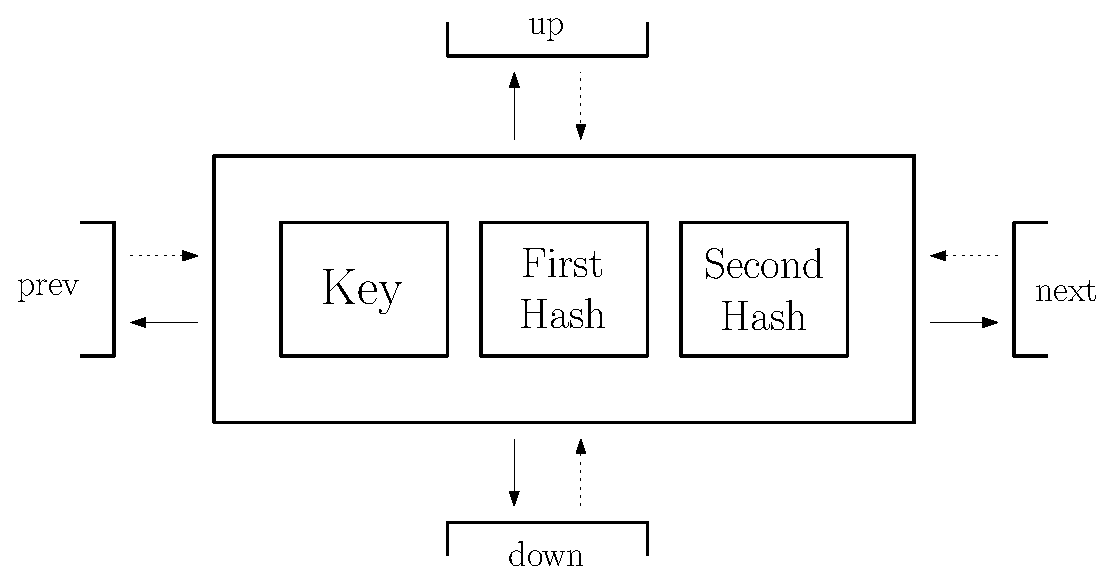
\includegraphics[scale=0.6]{figure/nodo.eps}
		\caption{Esempio di un nodo.}\label{fig:1}
	\end{figure}
		
	\subsection{Skip List Autenticata}
	
	%	MODELLO FUNZIONALE, motivare la realizzazione
	%	
	% 	Fatte tutte le opportune premesse descritte e motivate (APS style), si passa ora alla descrizione della struttura principale
	
	Prima di addentrarsi dettagliatamente su aspetti di natura progettuale e algoritmica della struttura dati autenticata, è necessario fare delle considerazioni di carattere generale, conseguenza di quanto detto in fase di analisi.
	Prima di tutto si sottolinea l'inutilità, in questo studio progettuale, della colonna di nodi sentinella di tipo $ +\infty $, la cui presenza comporterebbe solo un inutile spreco di memoria. I nodi sentinella di tipo $ -\infty $, d'altro canto, servono sia per poter avere una colonna che sia concettualmente antecedente a tutte le altre colonne presenti nella struttura e sia di supporto all'applicazione dello schema di hashing.
	Secondariamente si è ritenuto superfluo, e puramente formale, il mantenimento di un livello superiore a tutti gli altri livelli, contenente soltanto agli estremi i nodi sentinella. Questo aggiungerebbe solamente una passo in più agli algoritmi di esecuzione delle operazioni. Nel contesto più ampio di una successiva applicazione di memorizzazione in persistenza della struttura, il mantenimento di questo livello superiore complicherebbe soltanto la conversione da formato ad oggetti a quello della base di dati.
	
	La ricerca in tempo logaritmico, cosi come le operazioni di inserimento, cancellazione o modifica, sono permesse dalle chiavi dei nodi, che dunque saranno ordinate: $ k_{-\infty} < k_{1} < k_{2} < \dots < k_{n} < k_{+\infty} $.
	
	\begin{figure}[tbp] 
		\begin{center}
			\begin{tabular}{c @{\hspace{1em}} c}
				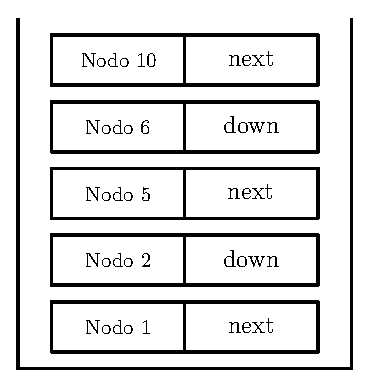
\includegraphics[scale=0.7]{figure/stack.eps} &
				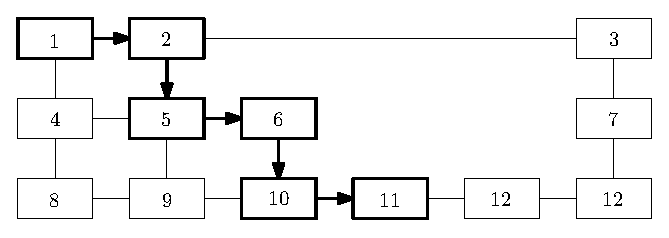
\includegraphics[scale=0.6]{figure/path.eps} \\
				(a) & (b)
			\end{tabular}
		\end{center}
		\caption{Esempio di una pila. I nodi sono stati volutamente segnati con un identificativo, per facilitare la comprensione dell'immagine, ma non hanno alcun riferimento con la progettazione o la realizzazione reale dei nodi. (a) La pila contenente in ordine di attraversamento, dal basso verso l'alto, i passi compiuti per comporre il \textit{path}. I blocchi della pila sono composti dal nodo di partenza di ogni passo, affiancato dalla stringa che indica la direzione del passo compiuto. (b) Sono evidenziati, nella Skip List, i nodi e le direzioni presenti nello stack, a seguito della ricerca dell'elemento 10.} \label{fig:stack+path}
	\end{figure}
	
	Segue la descrizione delle operazioni fornite, con enfasi sulle caratteristiche algoritmiche:
	
	\begin{itemize}
		\item \verb!getWithProof(k: String): Pair<Any?, Proof<ByteArray, String, Any>>!. L'algoritmo alla base di questa funzione, può essere diviso in due parti. La prima parte effettua una semplice ricerca di $ k $ sulla base delle chiavi contenute nei nodi, costruendo contemporaneamente la pila, \textit{stack}, di cui un esempio è raffigurato in figura \ref{fig:stack+path}. Questa funzione, come tutte le operazioni di read offerte dalla Skip List Autenticata, si appoggiano su una serie di metodi per la ricerca, che oltre a restituire il nodo cercato, riempono la pila con opportuni dati per ogni passo effettutato. La seconda parte sfrutta proprio il contenuto di questa pila, per poter costruire la \textit{Proof} relativa alla chiave cercata $ k $. Infatti il contenuto della pila, analizzato a ritroso rispetto all'ordine di riempimento, rappresenta il percorso, \textit{path}, inverso, dal nodo allo \textit{start node.}. Per costruire la Proof necessaria ad ottenere il \textit{root hash}, bisogna però "integrare" i nodi presenti nello stack, proprio per costruzione dello schema di hash adottato sulla struttura. Se, ad esempio, un nodo ha come \textit{next} un \textit{plateau}, allora esso dovrà essere inserito nella \textit{Proof} in quanto sarà necessario nella computazione degli hash. Lo stesso vale per i nodi \textit{down} di ogni nodo, che non siano presenti già nel \textit{path}.
		In base a quanto detto, una volta effettuata la ricerca dell'elemento, che indirettamente costituisce la pila, viene ripercorso il \textit{path} a ritroso partendo dall'elemento trovato, con opportune operazioni di pop. Ogni operazione di pop fornisce il successivo nodo presente nel \textit{path} e la direzione, in senso inverso, che deve essere intrapresa per raggiungerlo. Tramite questa seconda informazione è possibile distinguere il caso in cui, seguendo il \textit{path}, è necessario proseguire verso sinistra o verso l'alto. Nel primo caso sarà necessario integrare la \textit{Proof} con il nodo \textit{down} del successivo nodo del \textit{path}. Nel secondo caso, invece l'integrazione avviene solo nel caso in cui il nodo \textit{next} del successivo nodo del \textit{path} sia un \textit{plateau}.
		
		\item \verb!getProof(keys: List<String>): Proof<ByteArray, String, Any>!. Questa funzione in qualche modo estende la precedente, dando la possibilità, in un solo round, di richiedere ed ottenere una Proof valida per un insieme di chiavi passato come parametro. Ovviamente la lista passata dovrà necessariamente contenere solo chiavi presenti nella struttura.
		Per raggiungere questo obiettivo, da un lato la struttura si preoccupa di creare le singole Proof, una per volta, per ogni singola chiave passata come parametro, in quanto, come già detto, è l'unica entità che conosce le informazioni necessarie a farlo. Dall'altro è mantenuta una Proof cumulativa, valida per tutte le chiavi nell'intervallo $ [k[0], k[corrente]] $. Pertanto appena è creata una nuova Proof viene integrata con la Proof cumulativa corrente, richiedendo a quest'ultima una \verb!union(proof: Proof<ByteArray, String, Any>)!. Questo procedimento prosegue fino all'avvenuta presa in considerazione dell'ultima chiave in $ keys $, e termina con la restituzione della Proof cumulativa, a questo punta valida per tutto l'insieme di chiavi passato per parametro.
		
		\item \verb!getValue(k: String): Any?!. Si tratta di una semplice operazione di \textit{retrieve}. Infatti restituisce un valore di tipo $ V $, associato alla chiave $ k $ passata come parametro. Se non è presente la chiave è restituito $ null $.
		
		\item \verb!applyDeltas(): ADS<ByteArray, String, Any>!. Questa operazione permette alla struttura di avere la capacità di aggiornarsi rispetto a richieste di update in arrivo dai client. Trattandosi di una operazione di scrittura, e dovendo innestarsi in un ambito di concorrenza già altrove menzionato, sarà necessario evitare di modificare direttamente lo stato della struttura. Dunque viene separato il momento della ricezione di particolari richieste di update dal momento della loro effettiva applicazione. In questo modo sarà possibile \textit{clonare} la struttura corrente e applicare su quest'ultima gli update. Gli update possono tradursi in primitive di tipo \verb!add(k: String, v: Any): ByteArray! nel caso si trattasse di aggiunte o modifiche, o di tipo \verb!del(k: String): ByteArray! nel caso si trattasse di cancellazioni, andando rappresentare dei \textit{delta}, ossia delle variazioni in potenza della struttura. Essi sono accumulati, mantenendone l'ordine di "arrivo" in una pila, con opportune operazioni di $ push $. A seguito dell'invocazione di \verb!applyDeltas()!, le istanze della pila vengono valutata una ad una singolarmente, in ordine cronologico, con operazioni di $ pop $, e applicate a un clone della struttura corrente. Sarà poi questo, comprensivo degli update, ad essere restituito.
		L'attuazione effettiva delle varie azioni presenti all'interno della pila, è scissa, con l'obiettivo di migliorare la coesione generale, tra l'operazione \verb!applyAdd(k: String, v: Any)! nel caso di aggiunte o modifiche, e l'operazione di \verb!applyDel(k: String)! nel caso di cancellazioni.
		Queste scelte rendono invariato lo stato della struttura di partenza, che sarà dunque passibile di calcoli e computazioni anche contemporaneamente all'applicazione di update.
					
		\item \verb!rootHash(): ByteArray!. Operazione che calcola e restituisce il \textit{Root Hash} dell'intera struttura. Lo \textit{Start node} conterrà in ogni istante, nel campo \textit{firstHash}, il contributo in termini di concatenzioni di hash crittografici dato da tutti gli elementi correlati al campo \textit{down}, e nel campo \textit{secondHash}, il contributo in termini di concatenazioni di hash crittografici dato da tutti gli elementi correlati al campo \textit{next}. Viene, a questo punto, restituito l'hash derivato dalla concatenazione dei campi \textit{firstHash} e \textit{secondHash}.
			
		\item \verb!isEmpty(): Boolean!. Questa operazione semplicemente restituisce \textit{true} se la struttura non contiene nessuna coppia chiave-valore, \textit{false} altrimenti.

%	  [Appunti di ragionamento su cloning ADS]		
		\item \verb!clone(): ADS<ByteArray, String, Any>!. Copia la struttura e ne restituisce una identica, tranne per i delta che \underline{non} vengono copiati. Il problema della clonazione è di non banale risoluzione. Infatti la Skip List Autenticata è a tutti gli effetti un grafo diretto ciclico. Una prima possibilità potrebbe consistere nel clonare ogni torre iterando sulla \textit{base list}, per poi preoccuparsi solo in un secondo momento dei collegamenti orizzontali. La struttura della Skip List però comporterebbe una scansione di tutte queste torri clonate per ogni nodo di ogni torre, operazione con costo computazionale molto elevato e non auspicabile. Richiederebbe inoltre la conoscenza, diretta o indiretta, dell'altezza di ogni singola torre. 
		Per motivi analoghi, è da escludere anche la soluzione simmetrica, che memorizza ogni livello orizzontale, per poi preoccuparsi solo in un secondo momento dei collegamenti verticali.
		La soluzione poi effettivamente adottata, consiste nell'utilizzo di \textit{Hash Map} di supporto, una per ogni livello della Skip List Autenticata, tutte di lunghezza pari alla dimensione della \textit{base list} della struttura e tutte contenenti \textit{entries} con tutte le chiavi della struttura. Iterando orizzontalmente su ogni livello, le Hash Map corrispondenti saranno riempite. A seconda del nodo scansionato, verrà aggiunto un riferimento a quest'ultimo nella \textit{entry} corrispondente nella Hash Map. Se per una determinata chiave non sarà presente il nodo corrispondente a quel determinato livello, verrà mantenuto il valore di quella \textit{entry} a null. Così facendo sarà possibile avere tutti i riferimenti ad ogni nodo, e allo stesso tempo conoscerne l'esatta collocazione reciproca. Sarà possibile poi clonare ogni singolo nodo, e sostituire il riferimento contenuto nei vari valori delle Hash Map con i vari cloni. A questo punto sarà necessario solo provvedere ai collegamenti, sia orizzontali che verticali. Per quanto riguarda i collegamenti verticali sarà sufficiente collegare tutti i nodi con stessa chiave su Hash Map corrispondenti a livelli adiacenti. Per quanto riguarda i collegamenti orizzontali sarà necessario collegare i nodi adiacenti all'interno di una stessa Hash Map, intervallati cioè da sole \textit{entries} con valori nulli.	
		
	\end{itemize}

%	\begin{figure}
%		\centering
%		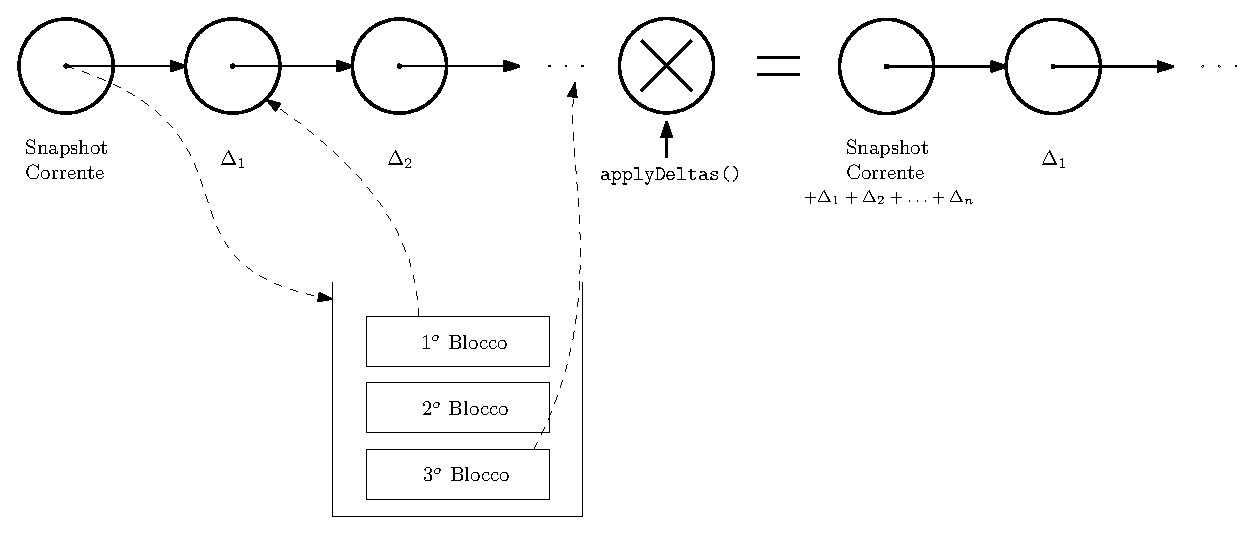
\includegraphics[scale=0.6]{figure/deltas.eps}
%		\caption{Schema che mostra il funzionamento dei \textit{delta}. Tramite primitive di tipo \verb!add(k: K, v: V)! e/o \verb!del(k: K)! si popola la pila della struttura con dei blocchi, ordinati cronologicamente. L'uso di \verb!applyDeltas()! applica in ordine questi \textit{delta} e restituisce un'altra struttura, con stato di partenza equivalente al primo \textit{snapshot}, ma con tutti i $\Delta_{n}$ applicati. La pila viene svuotata, ed è dunque poi pronta ad accogliere nuovi \textit{delta}.}\label{fig:delta}
%	\end{figure}

	\begin{figure}
		\centering
		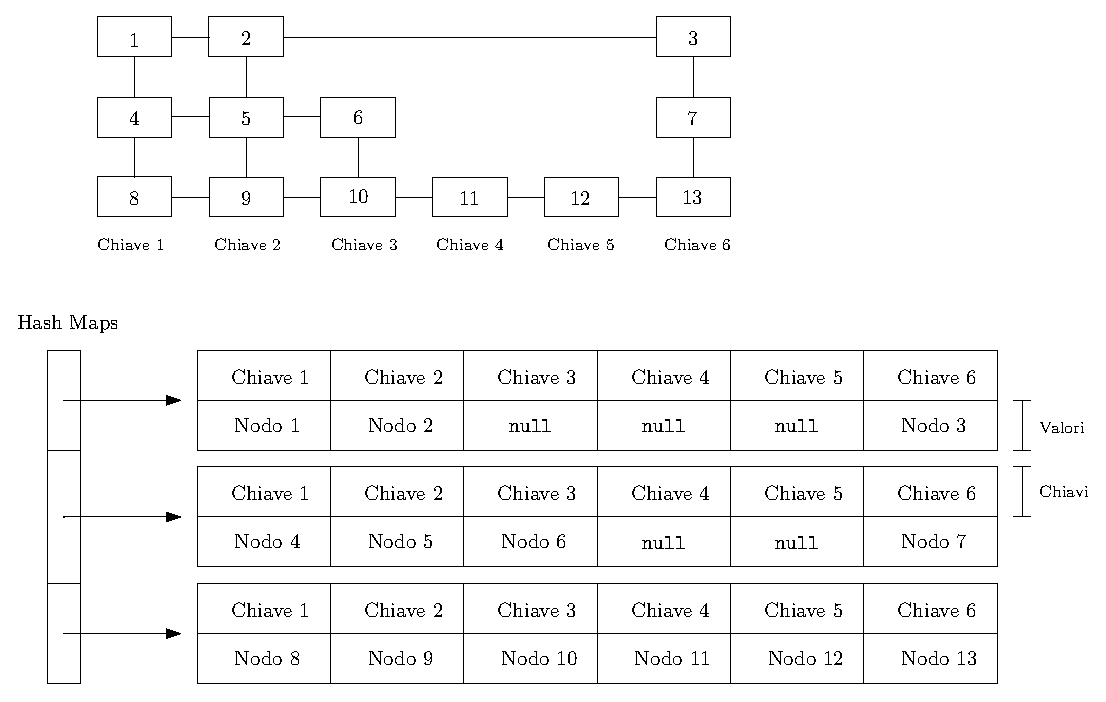
\includegraphics[scale=0.6]{figure/cloneADS.eps}
		\caption{Immagine che illustra un esempio di Hash Map, come sarebbero nella prima fase dell'operazione di clonazione, rispetto alla Skip List nell'esempio. E' possibile poi da questo stato clonare tutti i nodi e provvedere alla sistemazione di tutti i collegamenti.}\label{fig:cloneADS}
	\end{figure}
	
	\subsection{Skip List Proof}
	
	%	MODELLO FUNZIONALE, motivare la realizzazione
	%	
	%	Fatte tutte le opportune premesse descritte e motivate (APS style), si passa ora alla descrizione della struttura skip list proof
	

		Prima di addentrarsi dettagliatamente su aspetti di natura progettuale e algoritmica della Skip List Proof, è necessario fare delle premesse. La Proof, come già detto, concettualmente parlando, è relativa ad un particolare istante temporale della struttura dati autenticata da cui è stata generata. Dunque dal momento in cui inizia ad esistere, acquisisce uno stato e questo sarà completamente indipendente dallo stato della struttura di partenza. Pertanto la Skip List Proof, sarà una struttura dati indipendente e parallela all'ADS di partenza, di cui, inoltre, non avrà nessuna conoscenza, per motivi in parte già comprensibili, e in parte motivati in seguito nella sezione dedicata alla persistenza.

		In base all'utilizzo dell'API, inoltre, nell'ambito del protocollo di integrità su dati nel Cloud (6), sarà necessario poter applicare update ricevuti dall'ADS, nella forma compatibile con la Proof, alla Proof stessa, come già detto indipendente dalla struttura da cui è stata generata.
		
%	  [Discorso su somiglianza con albero]
		Fatti questi ragionamenti di natura concettuale, ora si riporta il ragionamento alla base di alcune decisioni progettuali e algoritmiche. La Proof per una chiave , rispetto alla Skip List Autenticata da cui è generata, è a tutti gli effetti poco più di un percorso, \textit{path}, dal nodo contenente quella specifica chiave, fino allo \textit{start node}. Gli elementi che ha in più sono i nodi necessari a ricostruire tutto il percorso di concatenazioni di hash necessarie a calcolare e restituire il \textit{Root Hash}, e sono o $ plateau $ presenti nel campo $ next $ di un nodo, non già presenti nel path, o nodi presenti nel campo $ down $ di un nodo, non già presenti nel path. La Proof cumulativa rispetto a un insieme di chiavi non fa altro che estendere la struttura corrente con ulteriori "path".
		Si potrebbe dunque pensare di rappresentare la Proof come fosse un albero binario, dove per ogni nodo, al posto di avere figlio destro e sinistro, si hanno rispettivamente nodo $ next $ e nodo $ down $. Tuttavia è facile dimostrare che la struttura sarebbe fortemente sbilanciata e risulterebbe oneroso computazionalmente, tra le varie foglie che si verrebbero a formare, trovare quali sono le chiavi per cui la Proof è valida, a meno che non si utilizzi una struttura dati di supporto per memorizzare i riferimenti a tali nodi. Rimarrebbe tuttavia non ottimale per quanto riguarda l'applicazione di aggiornamenti alla struttura.
 				
%	  [Discorso per giungere alla somiglianza con skip list] ==> [Motivare il nome del paragrafo e dunque della struttura]
		Si è preferito dunque utilizzare una struttura dati \textit{ad hoc}, con forti somiglianze con la Skip List Autenticata. I nodi e l'organizzazione interna saranno dunque uguali alla controparte. Le differenze principali risiedono nell'utilizzo di molti meno puntatori inter-nodo e nell'assenza di qualsiasi riferimento ai valori dello storage classico, prerogativa esclusiva dell'ADS. I nodi corrispondenti alla \textit{base list} avranno conoscenza solo dell'hash di questi valori.
		In questo modo inoltre, molte delle proprietà caratteristiche della Skip List, sarebbero ereditate da questa struttura, chiamata per ovvi motivi, \textit{Skip List Proof}, da cui il titolo del paragrafo.
		
%     [Discorso su scelta tra opzione HEAD e opzione KEYS]  ==> [Menzionare che lo start node è lo stesso della skip list autenticata]
		Riguardo la gestione interna della struttura, si individuano due principali alternative. La prima consiste nell'utilizzare come punto di partenza per ogni operazione il nodo \textit{HEAD}, corrispondente allo \textit{start node} della Skip List Autenticata. La seconda invece consiste nell'avere una struttura contenente i riferimenti ai nodi contenenti le coppie chiave-valore per le quali è valida la Proof. La seconda soluzione presenta dei vantaggi soprattutto per quanto riguarda le operazioni che devono essere effettuate su un specifiche chiavi, in quanto sarebbe possibile sostituire l'operazione di ricerca vera e propria, con un veloce accesso indicizzato. Tuttavia, come soluzione, risulterebbe svantaggiosa per tutti i calcoli che riguarderebbero il nodo \textit{HEAD}, in quanto non sarebbe presente un riferimento fisso a quest'ultimo. La soluzione poi realmente adottata è un ibrido tra le due. Sarà dunque utilizzato il riferimento al nodo \textit{HEAD} per le operazioni \verb!rootHash(): ByteArray! e \verb!union(proof: Proof<ByteArray, String, Any>): Proof<ByteArray, String, Any>! e la struttura proposta nella seconda soluzione, per ridurre di un fattore $\mathcal{O}(m)$ la complessità computazionale dell'operazione \verb!rootHash(list: List<Pair<String, Any?>>): Pair<Proof<ByteArray, String, Any>, ByteArray>!, la quale nel caso di adozione esclusiva della prima soluzione sarebbe dell'ordine di $\mathcal{O}(m^{2}*n)$, dove $ m $ è il numero di nodi nel \textit{path} di ogni singola Proof, e $ n $ è il numero di chiavi per cui è valida la Proof stessa.
		
						
		Segue la descrizione delle operazioni fornite, con enfasi sulle caratteristiche algoritmiche:
		
		\begin{itemize}
%			\item \verb|findNode(key: String, start: Node<K, H>? = null): Node<K, H>|. E' un operazione di ricerca. Intuitivamente, per costruzione di Skip List Proof, è analoga ai metodi di ricerca all'interno della Skip List Autenticata. Partendo dall'\textit{HEAD} o dal nodo $ start $ se passato per parametro, in base alla chiave $ key $ è effettuata la ricerca del nodo corrispondente. Se la chiave inserita non è presenta è necessario sia sollevata un'eccezione, altrimenti viene restituito il nodo trovato. Questa operazione è privata e di supporto alle successive operazioni, nel caso di sola adozione della soluzione con nodo \textit{HEAD}.
			
			\item \verb!rootHash(): ByteArray!. L'operazione è analoga a quella della Skip List Autenticata appena descritta. Calcola e restituisce il \textit{Root Hash} dell'intera proof. Il nodo \textit{HEAD} conterrà in ogni istante, nel campo \textit{firstHash}, il contributo in termini di concatenzioni di hash crittografici dato da tutti gli elementi correlati al campo \textit{down}, e nel campo \textit{secondHash}, il contributo in termini di concatenazioni di hash crittografici dato da tutti gli elementi correlati al campo \textit{next}. Viene, a questo punto, restituito l'hash derivato dalla concatenazione dei campi \textit{firstHash} e \textit{secondHash}.
			
			\item \verb!rootHash(list: List<Pair<String, Any?>>): Pair<Proof<ByteArray, String, Any>, ByteArray>!. Nel caso in cui tutti i valori passati siano nulli, l'operazione risulta equivalente a \verb|rootHash(): H|. Tramite la presenza di anche un solo valore non nullo, l'operazione diventerà di scrittura. Trattandosi di una operazione di scrittura, e dovendo innestarsi in un ambito di concorrenza già altrove menzionato, sarà necessario evitare di modificare direttamente lo stato della struttura. Dunque la struttura sarà clonata internamente e le modifiche agli hash saranno applicate sul clone. La struttura iniziale sarà dunque passibile di calcoli e computazioni anche contemporaneamente all'applicazione di queste modifiche. Il parametro che accetta è una lista di coppie chiave-valore, struttura che verrà processata iterativamente, rendendo superflua l'applicazione di una mappa di coppia chiave-valore. Nello specifico l'operazione processerà, per ogni chiave presente nella lista $ list $, il nodo corrispondente nella Proof, aggiornando gli hash, risalendo fino al nodo \textit{HEAD}. Al termine di questo elenco di queste operazioni, la funzione restituirà la nuova Proof, con le modifiche applicate e il nuovo \textit{Root Hash}.
			
			\item \verb!union(proof: Proof<ByteArray, String, Any>): Proof<ByteArray, String, Any>!. Trattandosi di una operazione di scrittura, e dovendo innestarsi in un ambito di concorrenza già altrove menzionato, sarà necessario evitare di modificare direttamente lo stato della struttura. Dunque la struttura sarà clonata internamente e l'unione verrà effettuta sul clone. L'unione consiste, intuitivamente, nell'integrazione della Proof su cui viene invocato il metodo, $ this $, con la Proof passata per parametro, $ proof $. Inizia, infatti, col trovare, tramite differenza tra insiemi, le chiavi presenti in $ proof $ che non sono presenti in $ this $. Per ognuna di queste chiavi risultato della differenza, se presenti, viene effettuata una iterazione parallela a partire dall'HEAD di $ this $ e dall'HEAD di $ proof $. che ha come fine quello di aggiungere a $ this $ i nodi per renderla valida per le ulteriori chiavi, contributo di $ proof $. E' mostrato in maniera più chiara nel seguente pseudocodice:
		
			\begin{algorithm}[H]
				\ForEach{key in (proof.keys - this.keys)}{
					first-iterator = this.head\;
					second-iterator = proof.head\;
					\If{second-iterator.next != null}{
						first-iterator.next = second-iterator.next\;
					}
					\If{second-iterator.down != null}{
						first-iterator.down = second-iterator.down\;
					}
					\eIf{second-iterator.next.key $ \leq $ key}{
						first-iterator = first-iterator.next\;
						second-iterator = second-iterator.next\;
					}{
						first-iterator = first-iterator.down\;
						second-iterator = second-iterator.down\;
					}
				}
			\end{algorithm}
			
%	      [Appunti di ragionamento su cloning Proof]			
			\item \verb!clone(): Proof<ByteArray, String, Any>!. Copia la struttura e ne restituisce una identica. La strategia utilizzata consiste nel clonare tutti i \textit{path}, uno ad uno, e successivamente creare la Proof cumulativa tramite \verb!union!. Dunque la complessità dovuta alla gestione del nodo \textit{HEAD}, in comune per tutti i path, e alla gestione dei "sotto-percorsi", ovvero insiemi di nodi comuni a più path, è spostata proprio su quel metodo. L'algoritmo alla base della clonazione di un path, consiste nel "risalire", con una sequenza di passi verso l'alto o verso sinistra, da ogni nodo contenente chiavi per cui la Proof è valida, fino al nodo \textit{HEAD} tenendo in considerazione l'eventuale presenza di nodi "fuori-path" necessari allo schema di hashing, inseriti perché, come già detto, necessari allo schema di hashing. Se infatti, nella risalita è effettuato un passo verso l'alto, sarà necessario controllare se il nodo da clonare ha un $ plateau $ nel campo $ next $. Se invece è effettuato un passo verso sinistra, bisognerà preoccuparsi di clonare l'eventuale nodo presente nel campo $ down $.
			
		\end{itemize}

	
\section{Persistenza}

%	Introduzione al discorso sulla persistenza, riallacciandosi a ciò che è stato detto nella parte di analisi. Descrizione del class diagram con pattern annessi

	Si passa ora alla sezione sulla \textit{persistenza}. Prima di tutto è necessario sottolineare che i ragionamenti per questa sezione sono stati effettuati prendendo in considerazione un particolare DBMS non relazionale, Cassandra. Tuttavia, a meno di piccoli accorgimenti, lo studio teorico che è di seguito condotto, è altamente flessibile rispetto alla tipologia di database NoSQL scelta.
	Da come è deducibile dal Class Diagram in figura~\ref{fig:services}, il progetto per il servizio di persistenza è stato pensato come una collaborazione attiva tra più parti, per mantenere alta la coesione globale.
	Il nucleo centrale è rappresentato dalla classe Pure Fabrication \textit{ADSService}. Questa funge da Controller per tutti i casi d'uso che necessitino di interagire con il database. Essa collabora con la classe \textit{CassandraConnector}, la quale interagisce direttamente con il database, e con \textit{Translator}, una classe di supporto per la conversione di formato dei dati scambiati con il database. E' previsto inoltre un sistema di \textit{Cache}, rappresentato dalla classe omonima, per massimizzare l'efficienza nello scambio di dati con il database.

	Nei successivi paragrafi si spiegherà più nel dettaglio ogni parte attiva all'interno del progetto di persistenza, illustrandone e motivandone tutte le scelte progettuali rilevanti.

	\subsection{Cassandra e NoSQL}
	
%	Sezione in cui si parla di Cassandra, in quanto un particolare tipo di database NoSQL e in funzione di questo paragrafo saranno affrontati tutti gli studi teorici e le scelte di progettazione

		Cassandra è un \textit{Database Management System} non relazionale e distribuito con licenza \textit{open source} e ottimizzato per la gestione di grandi quantità di dati. Fa parte della categoria di database NoSQL, ovvero di quei database dove la persistenza dei dati segue un meccanismo sostanzialmente diverso da quello appartenente al modello relazionale.  Tuttavia, rispetto allo standard dei NoSQL, garantisce consistenza e supporta il sistema di transazioni, entrambe caratteristiche molto importanti nell'ambito della memorizzazione in persistenza della struttura dati autenticata. Le componenti principali di Cassandra, di interesse per questa introduzione, sono le seguenti:
		
		\begin{itemize}
			\item \textbf{Nodo}: Luogo dove sono memorizzati i dati.
			\item \textbf{Centro dati}: Insieme di nodi correlati.
			\item \textbf{Cluster}: Componente che contiene uno o più centri dati.
		\end{itemize}
	
		Si tratta di un sistema \textit{masterless}, ovvero tutti i nodi all'interno di un Cluster sono organizzati secondo uno schema ad anello e svolgono lo stesso ruolo, ovvero sono identici e contengono ognuno una replica dei dati. Ognuno di essi può dunque rispondere alle richieste di lettura e/o scrittura, al pari degli altri. Questo garantisce l'assenza di un \textit{single point of failure}. Allo stesso tempo però tutti i nodi all'interno di un cluster sono interconnessi, in base al \textit{Gossip Protocol}, garantendo la continuazione di servizio nel caso in cui uno o più nodi dovessero essere fuori uso.
		
		Dal punto di vista logico, l'elemento più esterno è il \textit{Keyspace}. Esso contiene liste di \textit{Column Families}, ed è per questo che Cassandra è detto \textit{column-oriented}. Una column family, a sua volta, è una collezione di righe, rappresentate da una \textit{Map<RowKey, SortedMap<ColumnKey, ColumnValue>>}, dove però ogni riga è di lunghezza variabile. Mentre nel modello relazionale uno schema è fissato a priori, e una volta definite le colonne per una tabella, per ogni riga dovrò avere lo stesso numero di elementi, Cassandra è \textit{schema-free}. Pertanto ogni riga potrà avere un numero variabile di colonne, modificabile nel tempo in base alle esigenze, offrendo altissimi livelli di flessibilità. Cassandra dunque non obbliga ogni riga ad avere tutte le colonne. 
		Questi sono gli aspetti necessari alla comprensione degli studi teorici che seguono.
				
	\subsection{Studi teorici di progettazione}
		
%		Qui viene affrontato il problema dal punto di vista teorico, con particolare attenzione a sottolineare i problemi teorici derivati dallo studio 
%		teorico operato per quanto riguarda la persistenza di una struttura dati su base di dati NoSQL. Qui darei un accento più teorico, mentre le 
%		scelte progettuali che ne possono derivare, le descriverei nelle successive sezioni.

		% PRIMA DI TUTTO COME RAPPRESENTARLA E CORRISPONDENZA DELLE RAPPRESENTAZIONI

		In base a quanto detto si analizza ora il razionale alla base della memorizzazione della Skip List Autenticata in persistenza. Bisogna subito dire che risulta necessario trovare una corrispondenza tra il mondo ad oggetti, in-memory, dove deve essere utilizzata la struttura dati, e il mondo in persistenza, dove questa è effettivamente memorizzata. Le due parti hanno differenti modalità di rappresentazione interna degli stessi elementi. Ad esempio un nodo, o una serie di nodi della struttura, possono tradursi in una serie di stringhe di caratteri nel database. Pertanto per stabilire questa corrispondenza è necessario poter convertire da un formato "ad oggetti" al formato compatibile col database e viceversa.
		Gli algoritmi alla base di questa conversione, tuttavia, variano a seconda di come vengono fatti corrispondere elementi in memoria, ossia insiemi di nodi, con elementi di Cassandra, da qui in poi per comodità definiti \textit{blocchi}. Ossia dipendono strettamente dalla tipologia di rappresentazione logica scelta per rappresentare la struttura dati.
		
		% SCHEMA VERTICALE
		Per esempio, una possibile strategia, prevede il raggruppamento di nodi, a comporre blocchi in memoria, in maniera verticale. Ossia viene fatta corrispondere ad ogni torre della Skip List Autenticata un blocco in memoria. Questo, in ambiente Cassandra, corrisponderebbe ad avere per ogni torre una riga di lunghezza pari al numero di elementi presenti su quella torre. Questo è reso possibile, come detto, dal fatto che Cassandra non impone vincoli sul numero di colonne per ogni riga.
		Il problema principale di questo sistema risiede pero nel fatto che, supponendo di necessitare della coppia chiave-valore presente nel nodo sulla baselist memorizzato nel blocco i-esimo, obbliga al caricamento e/o restituzione di almeno tutti i blocchi dal primo fino all'i-esimo\footnote{Potrebbe essere necessario richiedere anche blocchi successivi all'i-esimo in quanto potrebbero memorizzare plateau fondamentali per ricostruire lo schema di hashing}.
		Altrimenti, nell'ottica del fatto che potenzialmente ogni blocco in memoria potrebbe corrispondere ad una query sia in lettura che in scrittura, è ragionevole pensare di voler ridurne il numero, aumentando il passo del blocco stesso. Dunque ogni elemento piuttosto che contenere una sola torre, potrebbe contenerne due o più. Questa soluzione tuttavia sebbene riduca il numero medio di query necessarie, dipendentemente dalla larghezza scelta per il passo, presenta sostanzialmente gli stessi problemi caratteristici di una schematizzazione verticale, la quale poco si confà alla natura della Skip List Autenticata, dal momento che elementi in alto a sinistra nella struttura saranno sempre o quasi sempre interessati dalle query. Con la memorizzazione verticale sarò obbligato sempre a restituire tutte le torri, anche se mi dovessero servire solo pochi singoli nodi.
		
		% SCHEMA ORIZZONTALE (dire che il blocco ha una sua struttura con max min e numero di elementi cosi come ivalori che contiene)
		Un'altra possibile strategia, invece, prevederebbe il raggruppamento di nodi secondo uno schema orizzontale. In questo caso, è opportuno anticipare che per definizione, la Skip List Autenticata, tende a crescere molto di più orizzontalmente che verticalmente. In particolare, sia $ n $ il numero di chiavi contenute, la dimensione orizzontale crescerà linearmente con l'aumento di $ n $, mentre l'altezza seguirà un trend logaritmico. Dunque, per motivi deducibili, non avrebbe senso avere blocchi orizzontali che ripercorrano l'intera lunghezza, ma essi dovranno essere segmentati. La segmentazione potrebbe essere simmetrica, ovvero i blocchi, di larghezza variabile ma fissabile a priori tramite limiti massimo e minimo di chiavi contenibili al suo interno, sono tutti incolonnati attraverso i vari livelli. Sebbene questa rappresentazione presenti interessanti proprietà probabilistiche, ha come principale difetto quello di non mantenere costante il numero di elementi per blocco. Il modo per ovviare a ciò è l'adozione di una strategia di segmentazione asimmetrica, dove quindi i blocchi avranno tutti la stessa larghezza, imponibile a priori, ma perderanno la possibilità di essere incolonnati. Per la strutturazione iniziale si può pensare che, poiché con alta probabilità ogni livello $ L_{i} $ avrà il doppio del numero degli elementi del livello $ L_{i+1} $, allora questa corrispondenza può riflettersi sui blocchi. Ed in particolare ogni blocco avrà un limite massimo e minimo e, almeno inizialmente, avrà in corrispondenza nel livello inferiore, esattamente due blocchi\footnote{Assunto che la probabilità di Coin Flip sia pari ad $ \frac{1}{2} $.}, i cui limiti massimo e minimo, divideranno esattamente il range del blocco sovrastante. In questo modo, lo schema dei blocchi, assomiglierà ad un albero binario. Questa struttura riesce a rendere tendenzialmente costante la dimensione del blocco, ma presenta dei problemi laddove i nodi, aggiunti randomicamente, formino una struttura molto discostata da quella dell'albero binario. Inoltre la asimmetria dello schema si andrebbe sempre più ad inacerbare nel caso di scritture che vanno ad aggiungere/rimuovere blocchi, o cambiarne i limiti massimo e/o minimo, complicandone la gestione dal punto di vista progettuale.
		
		% Si osserva che bisogna fare un trade-off per quanto riguarda la dimensione del blocco nell'ipotesi in cui mi preoccupo delle query
		Si osservi che un tratto comune nelle soluzioni sopra proposte riguarda la scelta della dimensione del blocco,, ovvero il numero di elementi contenuti, e dunque per costruzione la larghezza. Si tratterebbe di un \textit{trade-off} dove da un lato al crescere del blocco, crescono l'entità del traffico dati di ogni query il numero di nodi inutili ai fini dell'esecuzione delle operazioni, mentre si riduce il numero di elementi da richiedere/caricare per operazione. Dall'altro un blocco più piccolo consentirebbe di raggiungere una grana più fine riducendo il numero di nodi inutili e l'entità del traffico dati per ogni query, richiedendo però più operazioni di restituzione/caricamento.
		
		% Saerbbe auspicabile minimizzare la dimensione degli elementi che transitano e il numero di elementi inutili. DEGENERE a nodo --> Grana fine
		Sarebbe auspicabile poter minimizzare la dimensione degli elementi che transitano in modo da poter minimizzare il numero di elementi inutili. Questo è permesso dall'assegnare ad ogni nodo della struttura, un blocco cassandra a lui dedicato. In questo modo sarà possibile operare solo ed esclusivamente con i nodi interessati, trattando solo con elementi utili ai fini di una operazione da eseguire.		
				
		% Questo massimizza però il numero di elementi in transito e quindi le query
		Questa soluzione tuttavia massimizza contestualmente il numero di elementi in transito per le query.
		
		% Sarebbe auspicabile renderle indipendenti l'una dall' altra per poterle fare in parallelo e ottenerle in un round unico
		Di conseguenza sarebbe auspicabile rendere le query indipendenti l'una dall'altra. Fare in modo cioè che una query non dipendesse dal risultato di quella precedente. In questo modo esse potranno essere lanciate in parallelo in modo da permettere il caricamento o la restituzione di tutti gli elementi necessari, in un solo round.
		
		% PROBLEMA DI COME OTTENERE LE COSE IN PARALLELO. Parli del caso sequenziale e arrivi al caso parallelo. Serve la struttura, ma questa nel caso complesso cambia. Quindi la struttura andrebbe o aggiornata o richiesta e ricalcolata ogni volta. Questo in linea teorica permetterebbe di effettuare query in parallelo. Problema che ho due round per ogni query, voglio arrivare a uno. Auspicabile che invece che lato client, si potesse fare lato server. UDF function e round diventa uno. Auspicabile delegare a chi conosce i blocchi, il calcolo della struttura e insieme la restituzione dei blocchi. Lato Server. Non serve neanche che si ricavi la struttura, perche opera direttamente sui blocchi e ti restituisce quelli necessari. Scripting lato server --> UDF in cassandra
		Tuttavia, la richiesta di blocchi in maniera parallela richiede qualche informazione aggiuntiva. Una prima possibilità riguarda la conoscenza della struttura dei blocchi, e dunque dei nodi, ovvero la loro collocazione reciproca. Tuttavia questa è soggetta a continui cambiamenti nel caso di scritture che comportino aggiunte, cancellazioni o modifiche di blocchi. Pertanto la struttura andrebbe tenuta aggiornata o, in alternativa, richieste e/o ricalcolata prima di ogni operazione. Questo in linea teorica permetterebbe di effettuare query in parallelo, ma piuttosto che avere un round per operazione, ne avrei due, uno dedicato appunto all'ottenimento della struttura.
		Ragionando su quanto detto, si nota che il problema risiede nel fatto che si vorrebbe estrapolare un dato, di per se derivabile dai blocchi in qualsiasi istante, e materializzarlo lato client. Questa operazione comporta inevitabilmente tutte le difficoltà nel tenere questo dato aggiornato. L'ideale sarebbe il lasciare la gestione della struttura a chi può ottenerla e usarla, o in generale conoscerla, in maniera diretta, cioè lato server.
		La soluzione sta nello spostare la complessità di questa operazione tutta lato server, inviando solo i dati necessari a quest'ultimo e delegando il compito di individuare i nodi necessari e restituirli ad uno script server-side. Nel caso specifico di Cassandra è possibile affidarsi alle \textit{User-Defined Function}, UDF, ovvero delle funzioni definite dall'utente, che possono essere applicate ai dati memorizzati in persistenza.
		
		% NELLO SPECIFICO DELL'UTILIZZO POI DEVO CONSIDERARE OP DI SCRITTURA E DI LETTURA, QUELLE DI SCRITTURA POSSONO ESSERE SEMPLICI O COMPLESSE. SE HO BLOCCO-NODO QUESTO è RISOLTO
		Entrando più nello specifico dell'utilizzo, ovvero delle operazioni da eseguire dell'API, si nota la compresenza di operazioni di scrittura e di lettura. Nel caso di blocchi contenenti più nodi, le operazioni di scrittura possono diventare molto complicate da gestire. Infatti una modifica può potenzialmente completamente stravolgere un blocco, sia nelle informazioni che contiene, sia nelle meta-informazioni\footnote{Si tratta di meta-dati come il numero di elementi contenuti, il limite massimo, il limite minimo, il livello a cui si trova il blocco, e cosi via.}, fino a rendere possibile cancellazioni o creazioni di nuovi blocchi. Far corrispondere un singolo nodo ad un blocco Cassandra, risolve questo problema riducendo drasticamente la complessità di gestione della struttura in persistenza.
		
		% CORRISPONDENZA TRA BLOCCO MEMORIA E BLOCCO CASSANDRA, E INFORMAZIONI AGGIUNTIVE EVENTUALI CHE QUESTO DEVE CONTENERE. Discorso sul Livello, che non è necessario. Discorso su chiavi e indicizzazioni interne alla persistenza. Immagine illustrativa di UNA DELLE POSSIBILITA' soprattutto per avvalorare la tesi che non serve il level perche lo deduco dalla sequenza di restituizione
		Si ragiona ora sulle informazioni, ed eventualmente meta-informazioni, che dovrebbe contenere un blocco Cassandra, nel caso in cui ad ogni nodo corrisponda un blocco. Chiaramente dovrà contenere i due valori presenti nei campi \textit{First Hash} e \textit{Second Hash} cosi come la chiave. Potrebbe inoltre essere necessario memorizzare le informazione relative al livello in cui si trova il nodo, cosi come ai suoi campi $ next $, $ prev $, $ up $ e $ down $. Anche se seguendo una opportuna collocazione dei blocchi in persistenza è possibile rendere superflua la presenza di queste informazioni nella maggior parte delle query, deducendole facilmente dalla sequenza di blocchi restituita, si rende necessaria la presenza di un'ulteriore informazione riguardante il livello di struttura in cui si trovano. Così facendo ogni blocco sarà completamente identificabile.
		
		\begin{figure}[tbp] 
			\begin{center}
				\begin{tabular}{c @{\hspace{1em}} c}
					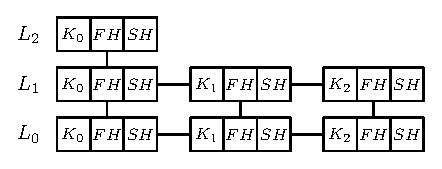
\includegraphics[scale=0.8]{figure/cassandra1.eps} &
					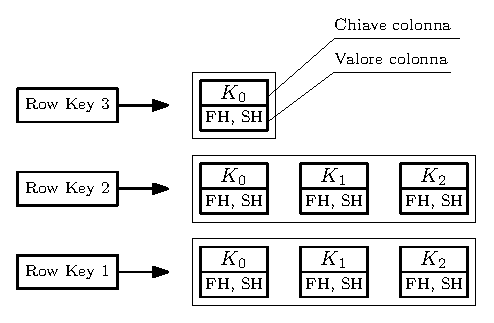
\includegraphics[scale=0.7]{figure/cassandra2.eps} \\
					(a) & (b)
				\end{tabular}
			\end{center}
			\caption{\textbf{(a)} Esempio di una Skip List Autenticata e \textbf{(b)} sua rispettiva possibile rappresentazione in persistenza su Cassandra. Ogni blocco, formato da una coppia chiave-valore di colonna, contiene le informazioni di un solo nodo.} \label{fig:bloccoCassandra}
		\end{figure}
		
		
	\subsection{Translator}
	
%	Entro nel dettaglio del Translator, descrivendo compiti e giustificandolo tramite pattern
	
		La conversione tra formato ad oggetti, in memoria, a formato in persistenza e viceversa, nel progetto precedentemente illustrato è affidata al \textit{Translator}. 
		
		Le operazioni che fornisce sono banalmente due, e sono simmetriche:
		\begin{itemize}
			\item \verb!translateToPersistence(ads: AuthSkipList<ByteArray, String, Any>): List<Block>! E' necessaria la conoscenza della logica di schematizzazione dei blocchi vigente all'interno del database. In questo modo è possibile preparare nell'esatta sequenza i blocchi che saranno poi caricati sul database.
			\item \verb!translateFromPersistence(blocks: List<Block>): AuthSkipList<ByteArray, String, Any>! Anche in questo caso è necessaria la conoscenza della logica di schematizzazione dei blocchi vigente all'interno del database. Infatti è possibile dedurre dai blocchi ricevuti dalla query, le informazioni necessarie a ricostruire la sezione di Skip List Autenticata. Come già detto infatti, in base all'operazione invocata sulla Skip List Autenticata, il Sistema provvederà a restituire soltanto i nodi che saranno toccati dall'operazione, ovvero solo quelli strettamente necessari all'esecuzione di quell'operazione.
		\end{itemize}
		
	\subsection{CassandraConnector}
	
%		Entro nel dettaglio del Connector, descrivendo compiti e giustificandolo tramite pattern

		Il \textit{CassandraConnector} ha il compito di stabilire la connessione vera a propria con il database, in base al particolare nodo e alla porta, entrambi specificati per parametro. Sarà dunque suo il compito di creare Keyspace e Tabelle necessarie alla memorizzazione della struttura dati, cosi come a fornire le primitive opportune per la gestione di operazioni di scrittura e lettura.
		
		Le operazioni principali che fornisce sono:
		\begin{itemize}
			\item \verb!connect(node: String, port: Integer)!. Stabilisce la connessione con il nodo $ node $ alla porta $ port $. Se non specificata, verrà utilizzata quella di default 9042.
			\item \verb!close()!. Chiude la connessione.
			\item \verb!createKeyspace(keyspaceName: String, replicationStrategy: String, replicationFactor: Int)!. Crea il Keyspace con nome $ keyspaceName $, fattore di replicazione dato da $ replicationFactor $ e strategia di replicazione data da $ replicationStrategy $. Questi due parametri stabiliscono il numero di repliche dei dati sui vari nodi e la strategia di distribuzione delle stesse all'interno dell'anello.
			\item \verb!createTable(List<String>)!. Crea la Column Family relativa alla struttura. Può accettare come parametro la lista di tutte le chiavi presenti nella struttura iniziale, che possono essere altrimenti aggiunte progressivamente.
			\item \verb!deleteKeyspace(keyspaceName: String)!. Elimina il Keyspace di nome $ keyspaceName $.
			\item \verb!deleteTable()!. Elimina la Column Family relativa alla struttura.
			\item \verb!storeADS(ads: String)!. Carica tutta la struttura passata per parametro. Funzione di utilità introdotta in base ad una specifica di utilizzo nell'ambito del protocollo, dove viene inizialmente creata una struttura iniziale, che dovrà dunque poter essere caricata in persistenza.
			\item \verb!selectPathForKey(k: String, filter: Filter): List<Block>!. Restituisce la sequenza di blocchi costituenti il $ path $ dallo \textit{Start Node} al nodo contenente la chiave $ k $.
			\item \verb!selectHead(): Block!. Restituisce i campi \textit{First Hash} e \textit{Second Hash} dello \textit{Start Node}.
			\item \verb!selectForAdd(k: String, filter: Filter): List<Block>!. Restituisce la sequenza di blocchi necessaria a poter eseguire un'inserimento o una modifica sulla struttura. Tiene conto dunque sia dell'eventualità di aggiunta di nuovi nodi, sia della modifica di nodi già presenti.
			\item \verb!selectForDel(k: String, filter: Filter): List<Block>!. Restituisce la sequenza di blocchi necessaria a poter eseguire una cancellazione sulla struttura. Tiene conto dunque sia dei nodi che saranno rimossi, sia di quelli che subiranno una modifica a seguito della rimozione di una torre.
			\item \verb!selectForProof(k: String, filter: Filter): List<Block>!. Restituisce la sequenza di blocchi necessaria per poter costruire la Proof relativa alla chiave $ k $. Questa funzione potrebbe essere utilizzata sia singolarmente per ottenere una Proof valida per una sola chiave, sia nell'ambito di una richiesta di una Proof cumulativa. In questo caso sarebbe necessario chiamare questa funzione tante volte quante sono le chiavi. E' possibile operare una ottimizzazione che restituisca la sequenza di blocchi necessari per poter ricostruire la Proof cumulativa per un insieme di chiavi. In tal caso la firma cambierebbe in: \verb!selectForProof(keys: Set<String>)!. 
			\item \verb!alterTableByAdd(structure: List<Block>)!. Effettua la sovrascrittura su database dei blocchi modificati e la scrittura di blocchi eventualmente aggiunti. Le informazioni relative all'aggiunta devono essere opportunamente codificate all'interno di una stringa di caratteri che sarà interpretata poi lato server.
			\item \verb!alterTableByDel(structure: List<Block>)!. Effettua la sovrascrittura su database dei blocchi modificati e la cancellazione di quelli rimossi. Le informazioni relative all'aggiunta devono essere opportunamente codificate all'interno di una stringa di caratteri che sarà interpretata poi lato server.
			\item \verb!containsKey(k: String): Boolean!. Restituisce true se la chiave è presente in struttura, false altrimenti.
		\end{itemize}
		
	
	\subsection{ADSService}
	
%		Entro nel dettaglio del Service, descrivendo compiti e giustificandolo tramite pattern.
%		Enfasi su come questa parte sia un centro-stella per le altre parti progettuali

		Come già deducibile da precedenti discussioni, l'\textit{ADSService} è un centro-stella per le altre parti progettuali. Essa, in base alle operazioni invocate sulla Skip List Autenticata, si occupa della cooperazione tra Translator e Connector per fornire le informazioni necessarie all'esecuzione delle operazioni stesse, da un lato, e per tenere aggiornata la struttura in persistenza, dall'altro.
		
		Le principali operazioni fornite sono:
			\begin{itemize}
			\item \verb!storeADS(ads: AuthSkipList<ByteArray, String, Any>)!. Funzione che permette il caricamento su database dell'intera struttura passata per parametro. La conversione di formato è delegata al Translator, e successivamente la sequenza ottenuta è passata al Connector che dovrà caricarla in persistenza.
			\item \verb!retrievePath(k: String): AuthSkipList<ByteArray, String, Any>!. Funzione che permette l'ottenimento della struttura necessaria a costituire un $ path $. Utile dunque per permettere le operazioni di ricerca e verifica di contenimento di chiave.
			\item \verb!retrieveForAdd(k: String): AuthSkipList<ByteArray, String, Any>!. Restituisce la struttura opportuna su cui potrà essere eseguita una modifica o una aggiunta sulla struttura.
			\item \verb!retrieveForDel(k: String): AuthSkipList<ByteArray, String, Any>!. Restituisce la struttura opportuna su cui potrà essere eseguita una cancellazione sulla struttura.
			\item \verb!getHead(): Node<String, ByteArray>!. Permette l'ottenimento dello \textit{Start Node}. Utile dunque per tutte le operazioni della Skip List Autenticata che necessitano solo di quest'ultimo.
			\item \verb!retrieveProof(Set<String>): AuthSkipList<ByteArray, String, Any>!. Permette l'ottenimento della struttura da cui sarà possibile ricavare la Proof cumulativa per un insieme di chiavi $ Set<String> $ passato per parametro.
			\item \verb!executeAdd(structure: AuthSkipList<ByteArray, String, Any>)!. Permette l'aggiornamento del database a seguito di una operazione di aggiunta/modifica effettuata sulla struttura.
			\item \verb!executeDel(structure): AuthSkipList<ByteArray, String, Any>)!. Permette l'aggiornamento del database a seguito di una operazione di cancellazione effettuata sulla struttura.		
			\item \verb!containsKey(k: String): Boolean!. Permette di verificare la presenza di una chiave nella struttura.
		\end{itemize}
		
	\subsection{Comportamento asincrono}
	
%		In base a quanto detto, sottolineare le decisioni progettuali e di come queste possano essere ottimizzate con
%		comportamento asincrono. Sottolineare bene che uno degli obiettivi è stato quello di minimizzare i round di 
%		query con Cassandra, e che questo è reso possibile da coroutine tipiche di linguaggi di programmazione OO moderni.

		In base ai ragionamenti condotti fin qui, è possibile operare una forma di ottimizzazione generale, data dall'introduzione di parallelismo sull'esecuzione delle varie query e/o operazioni. Infatti potrebbero essere frequenti situazioni in cui sarebbe possibile fare chiamate asincrone su varie funzioni la cui esecuzione parallela non creerebbe collisioni. Un esempio è il caso di letture parallele: le operazioni di lettura non modificano in alcun modo la struttura, pertanto possono essere distribuite su più thread di esecuzione paralleli. In questo caso le operazioni consisterebbero in una serie di chiamate asincrone annidate. Per gestirne opportunamente il flusso è necessario fare uso delle \textit{promesse} di restituzione futura di un valore, per poter gestire il responso delle varie esecuzioni.
		
	\subsection{Caching}
	
%		In questa parte si analizza il problema di caching. Descrivere compiti e giustificazioni
%		tramite pattern e future proofing. Giustificare anche in funzione del contesto piu generale delle dimensioni dell'ADS (fare calcolo su stime)

% 	 	LRU

		All'interno del progetto di persistenza è stato introdotto anche un sistema di \textit{caching} dei blocchi. Si è ipotizzato di applicare una \textit{Replacement policy} di tipo LRU, ovvero \textit{Last Recently Used}. Separatamente per ciascun blocco in cache è associato un \textit{replacement index}, ovvero un "contatore di età". I blocchi aventi il più alto valore saranno eliminati dalla cache, per fare spazio ad altri blocchi. Inoltre, ogni volta che un blocco di cache è acceduto il suo contatore è settato a zero, mentre gli altri contatori degli altri blocchi sono aumentati di 1, ad esclusione dei blocchi contenenti nodi direttamente adiacenti al blocco acceduto. La decisione del valore massimo di età, ovvero di una soglia massima di permanenza di un blocco in cache, è un valore variabile. All'aumentare della soglia, chiaramente, aumenteranno le probabilità di cache hit, a discapito di più spazio di memoria utilizzato.
		All'interno di questo progetto la cache viene riempita a seguito di una query di qualsiasi tipo. Le query che comportano scritture su database, devono preoccuparsi di aggiornare anche i blocchi in cache che hanno modificato.
		Tuttavia risulta necessario informare lo script server-side, in qualche modo, riguardo gli elementi già presenti in cache, che dunque non dovranno essere restituiti. Questo può essere risolto, aggiungendo alle query di tipo retrieve i blocchi già posseduti.
		

	\subsection{Bloom Filters}
	
% 	Sezione che illustra l'ottimizzazione per complessita di query su gestione caching

		Cosi facendo tuttavia, le query in uscita dal client hanno una lunghezza che è di ordine $\mathcal{O}(n)$ rispetto ai blocchi posseduti in cache. Si può allora prendere in considerazione l'adozione di \textit{Bloom Filters}, per passare informazioni al database riguardo la cache locale in $\mathcal{O}(1)$.
		Un Bloom Filter è una struttura dati probabilistica usata per testare se un elemento è o meno presente all'interno di un insieme. Sebbene siano presenti falsi positivi, è esclusa la possibilità di falsi negativi. In altre parole, una richiesta può risultare in un "possibilmente presente" o in un "sicuramente assente". Questo ben si adatta al caso di studio della cache, in quanto è perfettamente accettabile ricevere un numero esiguo di blocchi in realtà già presenti in cache. Non sarebbe invece stato accettabile il caso in cui sarebbero stati possibili falsi negativi, col rischio dunque di non ottenere blocchi invece necessari.
		Un Bloom Filter senza elementi è un array di $ m $ bit, tutti settati a 0. Possiede anche $ k $ differenti funzioni crittografiche di hash, ognuna delle quali "mappa" gli elementi dell'insieme a una delle $ m $ posizioni dell'array, generando una distribuzione randomica uniforme. Per aggiungere un elemento, bisogna farlo passare per le $ k $ funzioni di hash, per ottenere dunque $ k $ posizioni sull'array. I bit relativi a queste posizioni saranno dunque settati a 1. Dunque il test sulla presenza di un elemento segue lo stesso \textit{iter}: se anche solo una delle posizioni ha il bit settato a 0, vorrà dire che l'elemento è assente, altrimenti è presente. La possibilità di falsi positivi è data dal fatto che uno o più bit settati a 1 rispetto ad un elemento $ i_{1} $, potrebbero essere in realtà stati settati dall'inserimento di un altro elemento $ i_{2} $, con $ i_{1}\ne i_{2} $.	
		Gli elementi dunque possono essere aggiunti all'insieme, ma non possono essere rimossi. Infatti una rimozione non è possibile, proprio dal fatto che falsi negativi non sono permessi. Settare a 0 anche solo un bit di un elemento, potrebbe comportare l'eliminazione di altri elementi mappati su quel bit.
		I Bloom Filter hanno inoltre l'importante proprietà, utile anch'essa ai fini dei questo studio di caso, secondo cui il tempo richiesto per aggiunte o per verificare la presenza di un elemento è costante, ed è $\mathcal{O}(k)$, ovvero è completamente indipendente dal numero di elementi nell'insieme. I $ k $ \textit{lookup}, inoltre, sono indipendenti tra loro, e potrebbero essere parallelizzati per aumentare l'efficienza.
		
		Dovendo tuttavia rispecchiare la cache presente in memoria, è necessaria la possibilità di cancellazione di un elemento, come detto impossibile per un semplice Bloom Filter. Sarebbe possibile l'utilizzo di una sua estensione, i \textit{Counting Filters}, che aggiungono esattamente quella caratteristica, tramite la promozione di ogni posizione dell'array da 1-bit ad n-bit. In questo modo l'operazione di inserimento non farà altro che incrementare il valore presente nella posizione, e la verifica di presenza controllerà che nelle $ k $ posizioni non ci sia un bit pari a 0. Tuttavia, se già i Bloom Filter classici, utilizzano $ 1.44\log{2}{\frac{1}{\epsilon}} $ bit di spazio per elemento inserito nell'insieme, dove $\epsilon$ è la probabilità di falso positivo della struttura, i Counting Filters utilizzano mediamende 3-4 volte lo spazio. Questo potrebbe dunque ridurne l'utilità di utilizzo all'interno del progetto di persistenza.
		Tuttavia una soluzione ottimale invece prevede l'utilizzo dei \textit{Cuckoo Filters} \cite{cuckoo}, ovvero una evoluzione dei Bloom Filters, che permettono sia aggiunte che cancellazioni, ma ottimizzate per l'utilizzo dello spazio. Infatti possiedono un algoritmo di riempimento dell'array più sofisticato in grado di garantire prestazioni molto superiori a quelle di estensioni classiche dei Bloom Filters.
		
		Dunque, in definitiva, il filtro passato nella query permetterà alla UDF server-side il check se un blocco è presente o meno in cache, e potrà dunque decidere se restituirlo o meno. In cache dunque sarà presente una lista di blocchi dove continuerà a valere quanto detto fin ora, accostata ad un Cuckoo Filter, sincronizzato con quest'ultima. 
		

	\subsection{Modello con attori}
	
%	Se si vuole considerare che nell'utilizzo pratico, attori presenti sul server operano in parallelo sulla struttura, per dare parallelismo è possibile inserire un attore per ogni nodo della struttura dati. Cosi si potrà accedere alla struttura dati da vari punti in modo parallelo. L'attore radice potrebbe essere un collo di bottiglia, ma posso dedicargli CPU esclusiva. Miglioria possibile riguarda l'avere un attore per le letture e uno per le scritture per ogni singolo nodo. Una volta caricata la struttura su Cassandra, poi per tutte le query successive, invece di passare per uno script lato server per individuazione, restituzione e scrittura dei nodi necessari, assegno ad ogni attore un nodo (cioè blocco cassandra) e poi per tutte le query passo per gli attori? Dove ogni attore quindi conosce il solo blocco a lui assegnato.
%	Basta che gli attori mantengano la struttura tra loro e si possono fare query parallele.

		Se si vuole inoltre considerare che, nell'utilizzo pratico, attori presenti sul server operano in parallelo sulla struttura dati, ovvero eseguono operazioni in maniera concorrente sulla stessa risorsa, è possibile introdurre una piccola estensione che si basa sull'utilizzo del modello ad attori. Il Modello ad Attori è una recente teoria di programmazione concorrente che consente la creazione di applicazioni sviluppate attorno a delle unità di processamento chiamate \textit{Attori}, e dove il processamento degli attori è descrivibile come un ciclo indefinito di ricezione e processamento di messaggi, primitiva di comunicazione tra attori.
		E' possibile dunque assegnare un attore per ogni nodo della struttura dati. Così facendo si potrà accedere alla struttura dati da vari punti in modo parallelo. L'attore radice, ovvero quello che corrisponderebbe allo \textit{Start Node}, potrebbe rappresentare un collo di bottiglia. Tuttavia essendo un caso circoscritto, è possibile dedicargli potenza di calcolo esclusiva. Una miglioria a questo sistema potrebbe consistere nell'avere due attori per ogni nodo della struttura, uno dedicato alle letture e uno alle scritture.
		Dunque, una volta caricata la struttura in persistenza, viene creata una corrispondenza biunivoca tra i blocchi cassandra e una serie di attori, i quali conoscono solo il riferimento al nodo a loro assegnato, ed inoltre si conosce la struttura reciproca degli attori stessi. Dunque a questo punto, invece di utilizzare una forma di scripting server-side per l'individuazione, restituzione e scrittura dei nodi necessari passo per questa rete di attori presente in memoria.
		Questo sistema consentirebbe inoltre di bypassare il sistema transazionale dei classici database, adattando le query in maniera ottimale alla natura della Skip List, che, come già detto in fase di analisi, è molto poco bloccante negli accessi paralleli. Infatti devono essere bloccati solo i blocchi interessati da una operazione di scrittura, mentre possono essere lasciati disponibili tutti gli altri blocchi. Inoltre, immaginando una sequenza di blocchi $ B_{0}, B_{1}, ..., B_{n} $ da processare all'interno di una query, in questo modo è facile immaginare un sistema di \textit{pipeline} in cui già dal momento in cui si sta processando il blocco $ B_{1} $, si rende libero il blocco precedente, e cosi via.

	\subsection{Progettazione}

%	Questa è la sezione in cui si parla di tutto il progetto legato alla persistenza, e di come questo si lega al tutto.
%	E' importante qui accennare tutti gli attori e la loro interazione globale. Il focus qui è sulle varie operazioni di sistema

% 	DIAGRAMMI DI SEQUENZA PER LE OPERAZIONI

	Seguono delle immagini per illustrare, sulla base di quanto detto, la collaborazione tra le varie parti per permettere la memorizzazione della Skip List Autenticata in persistenza e contestualmente l'utilizzo dell'API. I diagrammi di sequenza sono costruiti in base alle operazioni eseguibili dalla Skip List Autenticata e mostrano come sia possibile rispettare il requisito della trasparenza di questa estensione rispetto alla libreria standard.\footnote{Si perdoni un piccolo abuso di notazione sui vincoli all'interno dei frame condizionali, attuato per favorire la comprensione del lettore.}

	\begin{figure}
		\centering
		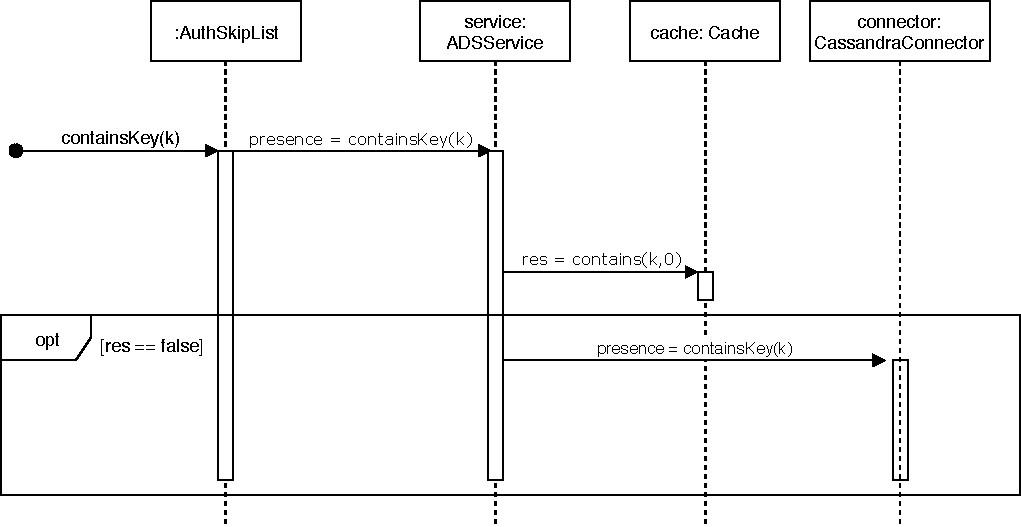
\includegraphics[scale=0.6]{figure/containsKeySD.pdf}
		\caption{Diagramma di sequenza per l'operazione di check sulla presenza di una chiave.}\label{fig:containsKeySD}
	\end{figure}

	\begin{figure}
		\centering
		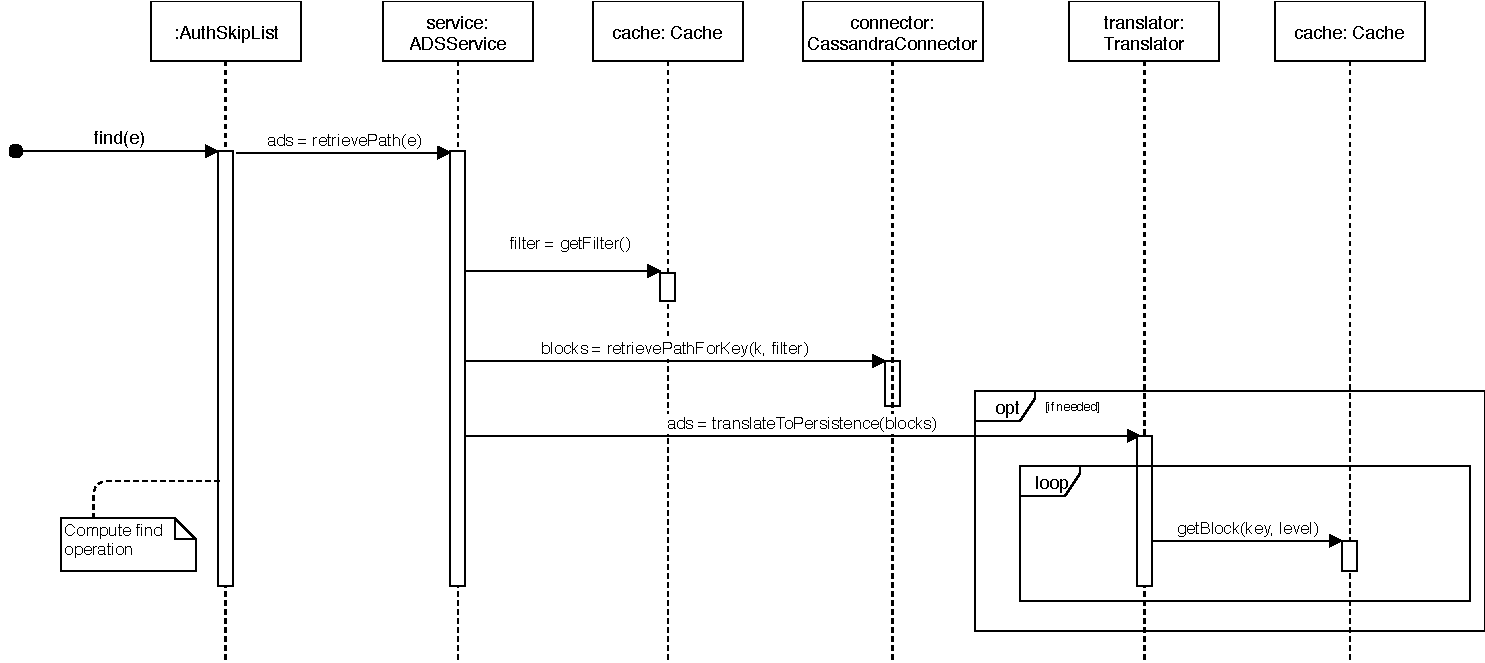
\includegraphics[scale=0.6]{figure/findSD.pdf}
		\caption{Diagramma di sequenza per l'operazione di ricerca di una chiave.}\label{fig:findSD}
	\end{figure}

	\begin{figure}
		\centering
		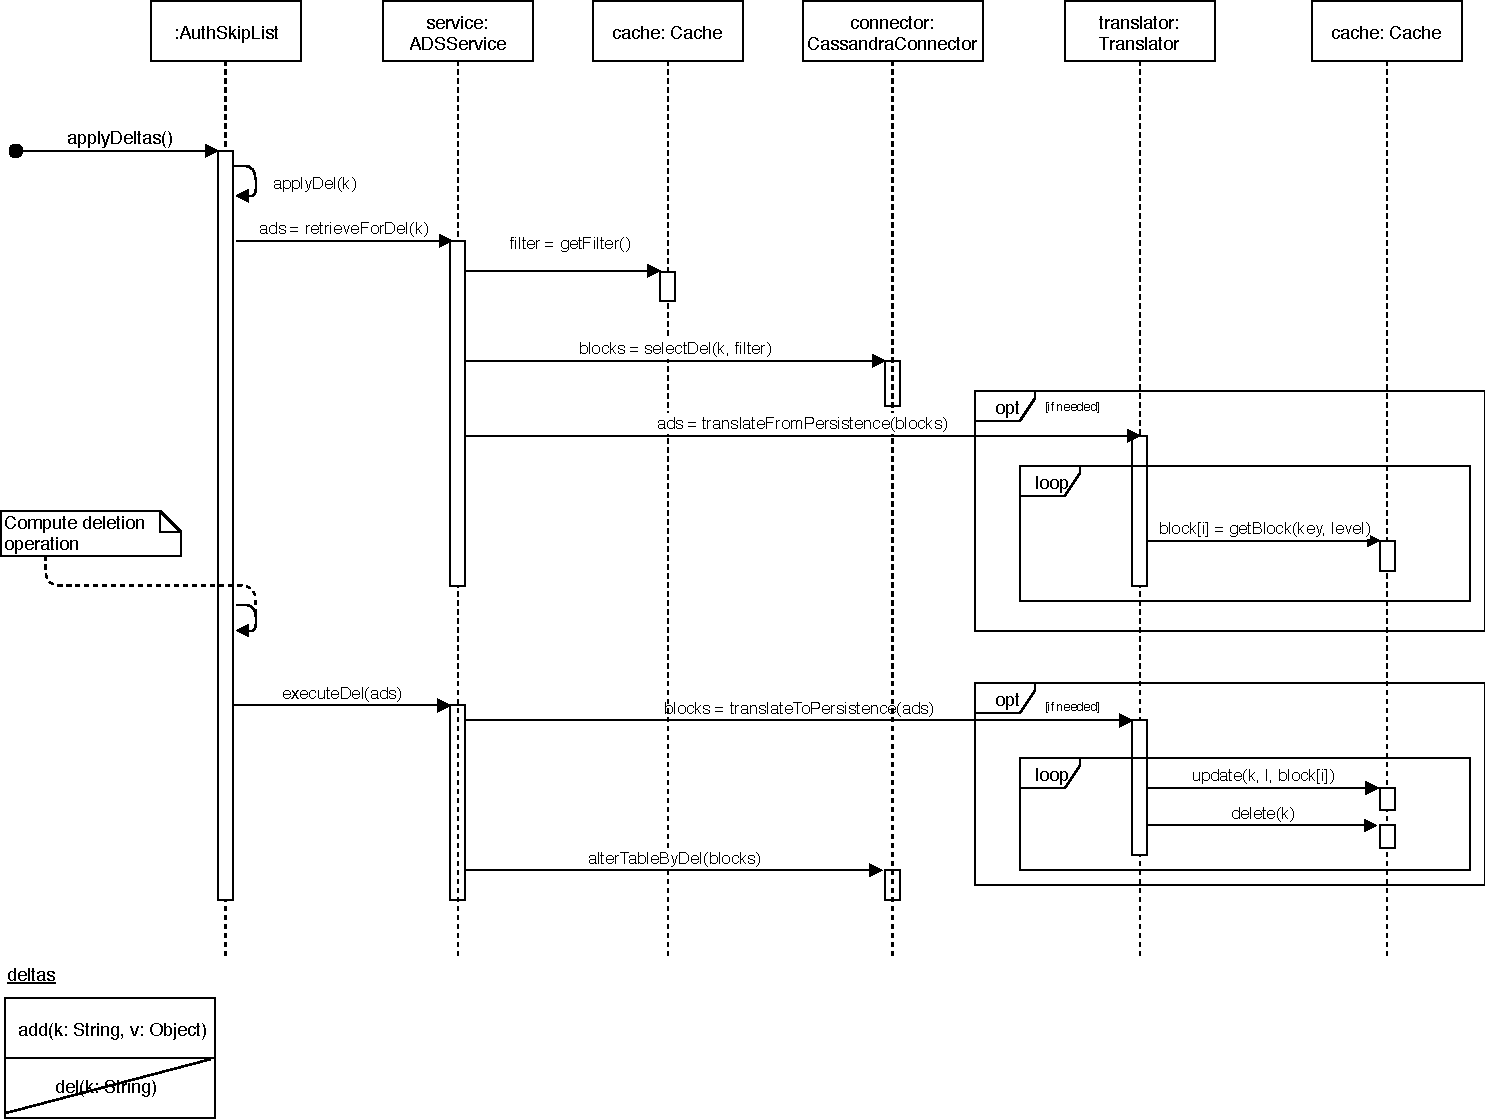
\includegraphics[scale=0.6]{figure/applyDeltasSD.pdf}
		\caption{Diagramma di sequenza per l'operazione di applyDeltas(). Lo schema mostra un particolare esempio in cui devono essere effettuate due operazioni, una di cancellazione e una di aggiunta. E' mostrata solo la parte di cancellazione in quanto la parte di aggiunta è analoga. La creazione di blocchi attuata dal Translator è implicita.}\label{fig:applyDeltasSD}
	\end{figure}

	\begin{figure}
		\centering
		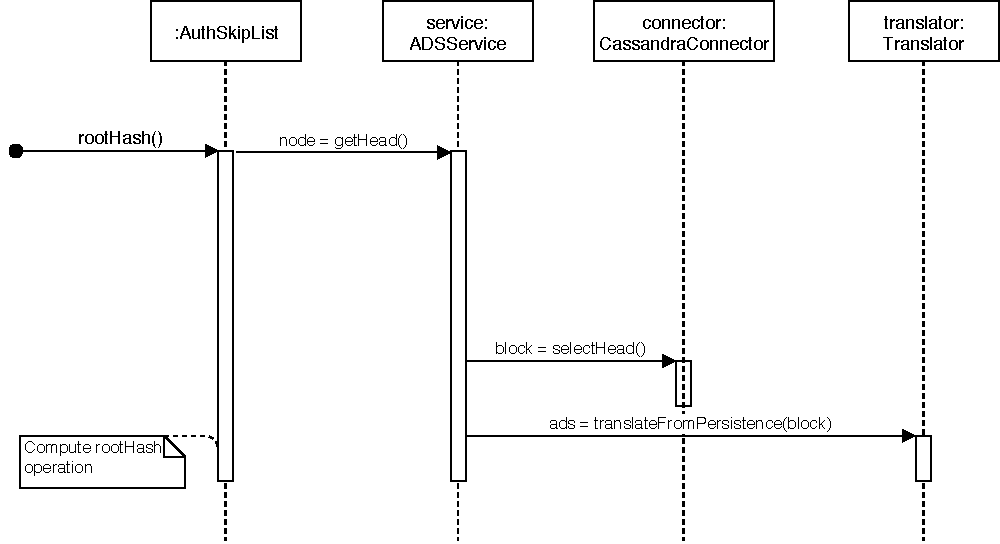
\includegraphics[scale=0.6]{figure/rootHashSD.pdf}
		\caption{Diagramma di sequenza per l'operazione di calcolo del Root Hash.}\label{fig:rootHashSD}
	\end{figure}

	\begin{figure}
		\centering
		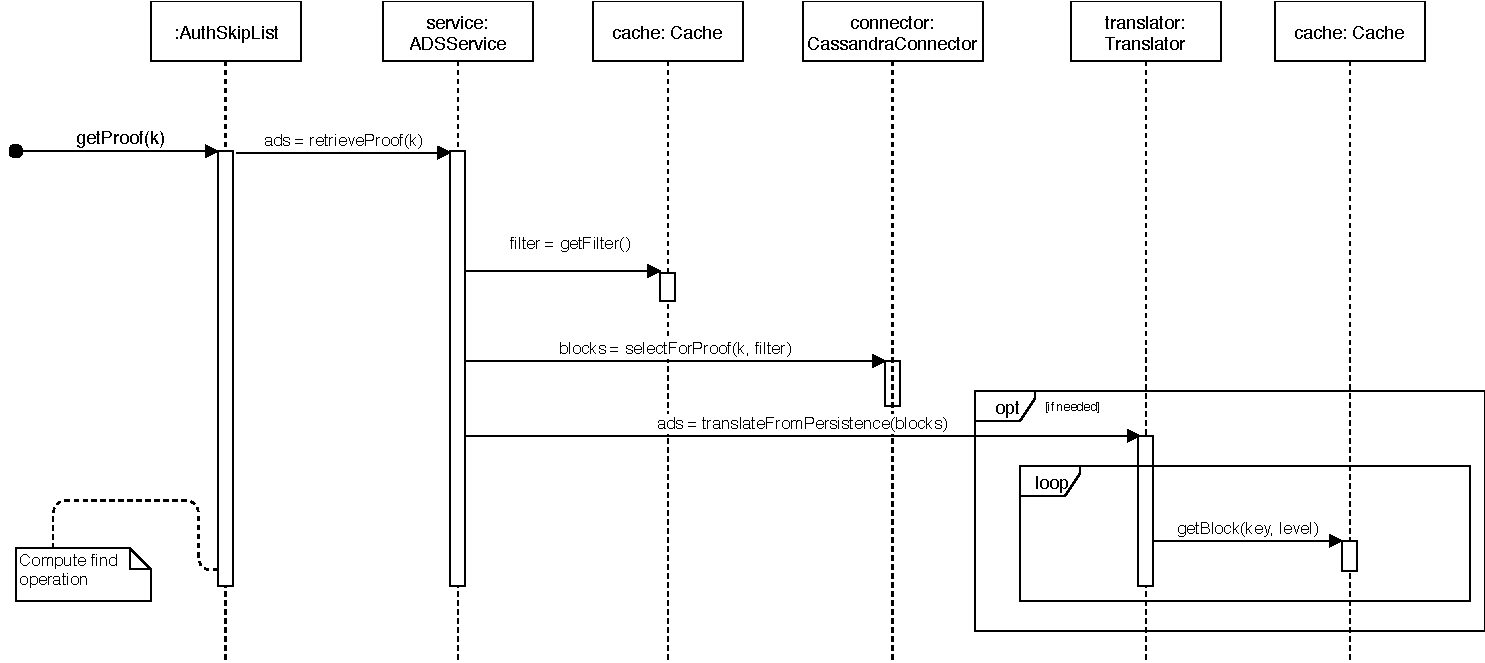
\includegraphics[scale=0.6]{figure/getProofSD.pdf}
		\caption{Diagramma di sequenza per l'operazione di ottenimento di una Proof valida per una chiave.}\label{fig:getProofSD}
	\end{figure}




